\documentclass[12pt,a4paper]{article}

\usepackage[T1]{fontenc}
\usepackage[utf8]{inputenc}
\usepackage[italian]{babel}

\usepackage{graphicx}
\usepackage{float}
\usepackage[margin=1in]{geometry}
\title{Business Intelligence e Big Data M}
\author{Alessio Reitano}

\makeindex

\begin{document}
	\maketitle
	\tableofcontents

	\newpage
	
	\listoffigures
	
	\newpage

	\section{La Business Intelligence}
Inizialmente \textbf{l’informatica} ha avuto un ruolo assolutamente secondario, il cui compito era quello di memorizzare \textbf{dati operazionali}, ossia tutti quei dati che vengono generati e memorizzati per tenere traccia delle operazioni che vengono svolte in un’azienda. (es. registrazione di una fattura, ordine di materiale). Tali dati sono chiamati anche \textbf{dati transazionali}.

Un \textbf{sistema informativo} è tutto il patrimonio di dati e informazioni raccolto e gestito in maniera coerente da un’azienda. Nel sistema informativo rientrano non solo i DB ma anche tutte le informazioni che stanno nella testa delle persone, nei documenti cartacei, nelle e-mail che vengono scambiate ecc. Un \textbf{DataBase} è una raccolta di dati coerenti, organizzati secondo un modello e memorizzata su un supporto informatico. \textbf{ Un modello} è una collezione di concetti che viene usata per descrivere i dati. Ad esempio, se si ha un database relazionale, avrò una collezione di dati organizzata in tabelle e quindi avrò un \textbf{DBMS relazionale} che gestisce quel DB, dove per “gestire” si intende scrive, legge e gestisce gli accessi degli utenti a questi dati. Nei DB quando si deve fare un’operazione, nello specifico facciamo riferimento ad una \textbf{transazione}, ovvero un insieme di operazioni elementari che non possono essere fatte singolarmente, in quando le transazioni sono da considerarsi azioni atomiche. Con il passare degli anni i sistemi informativi si sono trasformati da semplici strumenti per migliorare l’efficienza dei processi, cioè più veloci, a elementi centrali dell’organizzazione aziendale, creando di per sé una ricchezza e influenzando il modo in cui fare business.
\begin{figure}[H]
	\centering
	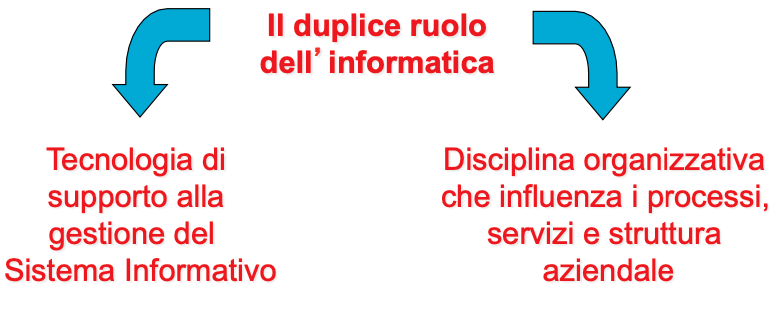
\includegraphics[width=0.9\textwidth]{img/Cursor_e_2-IntroDW_pdf}
	\caption{Ruolo dell'informatica}
	\label{fig:cursore2-introdwpdf}
\end{figure}

In questo corso, affronteremo in modo particolare il \textbf{processo decisionale}, in quando ci collochiamo ad un livello alto dell’organigramma. A noi non interessano gli impiegati, ovvero il livello medio-basso, ma i manager, cioè coloro che nell’azienda devono prendere decisioni. Nel processo decisionale il ruolo dell’informatica diventa ancora più importante. Per esempio, nel caso in cui un’azienda (Fiat o Lamborghini), volesse aprire un nuovo stabilimento bisognerebbe prendere una decisione basata sul \textbf{data driven} (guidata dai dati). Di conseguenza ho bisogno di un sistema informatico che mi aiuti nel processo decisionale.

\begin{figure}[H]
	\centering
	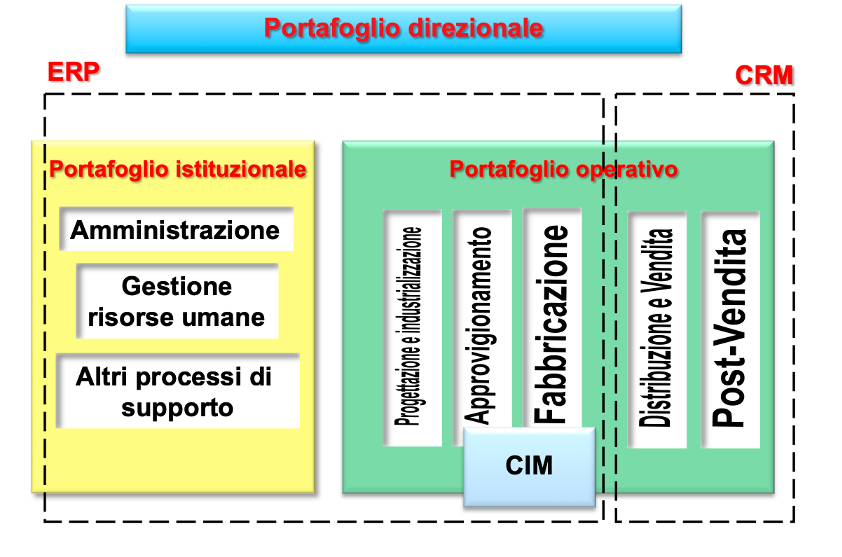
\includegraphics[width=0.7\textwidth]{img/portafoglio}
	\caption{Portafoglio Direzionale}
	\label{fig:portafoglio}
\end{figure}
Il \textbf{portafoglio direzionale} rappresentato in figura \ref{fig:portafoglio} è l’insieme delle applicazioni utilizzate dai manager aziendali per:
\begin{itemize}
	\item 
	Analizzare lo stato dell’azienda
	\item 
	Prendere decisioni rapide
	\item 
	Prendere le decisioni migliori
\end{itemize}
ed è costituito da due parti:
\begin{enumerate}
	\item 
	\textbf{ERP (Enterprise Resource Planning)}: non sono un DBMS pur gestendo dati. Coprono un’area molto vasta del business aziendali, come quella del portafoglio istituzionale e parte del portafoglio operativo e hanno caratteristiche particolari come:
	\begin{itemize}
		\item
		l’unicità del dato
		\item 
		concetto di configurazione, che permette di adattarsi in parte ai 
		requisiti della specifica azienda
		\item 
		modularità, compro solo alcuni moduli dell’ERP
	\end{itemize}
	
	Uno degli ERP più noti è \textbf{SAP}.
	
	\item 
	\textbf{CRM (customer relationship manager)}: simile all’ERP ma in ambito diverso, è più orientato al cliente. Il caso più banale è quello degli operatori telefonici che per proporre delle offerte hanno sotto un CRM, il quale indica i potenziali clienti. 
	
\end{enumerate}
Tutta la parte sotto la linea tratteggiata sono dati operazionali, i quali saranno il nostro punto di partenza.

Tipicamente si parla anche di piattaforma di \textbf{Business Intelligence}, ovvero un insieme di strumenti e procedure che consentono a un’azienda di trasformare i propri dati di business in informazioni e conoscenza utili al processo decisionale. L'\textbf{informazione} è una specie di distillato dei dati, perché abbiamo una maggiore qualità dei dati, gli errori sono stati corretti e  si è rinunciato ad un livello di dettaglio che magari non interessava per il processo decisionale. La \textbf{conoscenza}, quantità ancora minore ma valore ancora più elevato, perché a partire dalla conoscenza si possono prendere decisioni e quindi agire all’interno dell’azienda. Informazione e conoscenza vengono affidate ai decisori aziendali per decidere quali strategie adottare per il business. L’obiettivo è trarre vantaggio rispetto ai \textbf{competitor}, migliorare le prestazioni, aumentare la \textbf{profitability}, e più in generale, \textbf{creare valore} per l’azienda.
Si parla di piattaforma di BI poiché per consentire ai manager analisi potenti e flessibili è necessario definire un’apposita infrastruttura hardware e software di supporto composta da:
\begin{itemize}
	\item 
	Hardware dedicato, avrò un server su cui gira tutta la "roba" della BI
	\item 
	Infrastrutture di rete
	\item 
	DBMS, fatto in modo da gestire grandi quantità di dati
	\item 
	Software di back-end
	\item 
	Software di front-end
\end{itemize}
Il ruolo chiave di una piattaforma di BI è la trasformazione dei dati in informazioni e quindi in conoscenza.

\subsection{La piramide della BI}

\begin{figure}[H]	
	\centering
	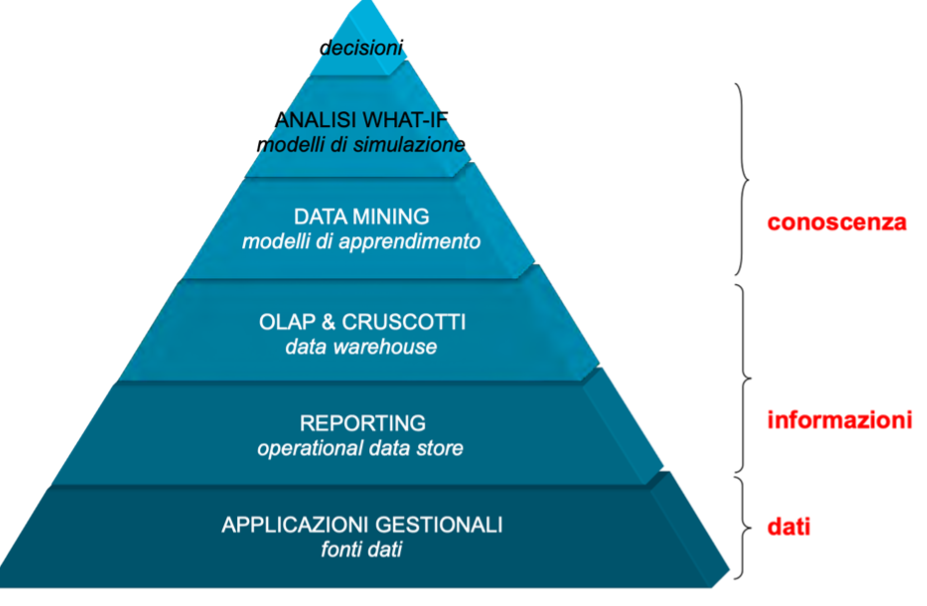
\includegraphics[width=0.7\linewidth]{img/piramide}
	\caption{Piramide della BI}
	\label{fig:piramide}
\end{figure}

Al livello più basso della piramide rappresentata in figura \ref{fig:piramide} troviamo i dati gestiti da applicazioni gestionali, cioè programmi. Per fare un esempio immaginiamo di essere un’azienda a cui serve un programma per fare le fatture in forma digitale, quindi usando un DB. I DB sappiamo che sono gestiti da un DBMS, ma non posso immaginare di fare interagire l’utente finale direttamente con un DBMS. Dunque, tra l’utente e il DBMS ho bisogno di uno strato applicativo che da un lato deve presentare delle finestre adatte ad un utente non tecnico e dall’altro deve essere in grado di parlare con il DBMS. 
Con i due livelli successivi entriamo nel mondo dell’informazione, in cui troviamo “l\textbf{’operational data store}” e il “\textbf{data warehouse}”. Il primo è un livello di database intermedio tra i due mondi, nel quale si trovano  dati dettagliati ma puliti. Nel secondo invece, ho proprio l’informazione, quindi vado ad effettuare la sintesi dei dati.

\textbf{L’operation data store}, in genere, lo uso per fare il reporting operativo, cioè per lanciare delle query che generano i cosiddetti “listoni”. Il livello di data warehouse è un repository, di natura completamente diversa rispetto a quello precedente, in cui l’interazione avviene attraverso un particolare paradigma di interrogazione, \textit{OLAP} e \textit{CRUSCOTTI} dashboard. Al livello del \textbf{DATA MINING}, si entra nel mondo della conoscenza. Gli strumenti di data mining implementano degli algoritmi complessi, in grado di estrarre conoscenza nascosta, in grosse quantità di dati, i cosiddetti pattern, ovvero schemi di comportamento che gli algoritmi di data mining riescono a portare alla luce. In particolare, tali algoritmi fanno uso delle regole associative. Ancora più in alto, troviamo l’\textbf{analisi what-if} (cosa-se). Ci si trova vicino alla cima, in cui sono presenti le decisioni. Se ho uno strumento che mi permette di prevedere, nel caso dell’esempio degli spinaci (offerta 3X2), se ci guadagno o ci perdo prendere una decisione diventa facile. Tutto ciò non è semplice da ottenere perché ci sono tanti fattori. 

Il \textbf{ciclo decisionale} in BI si articola in quattro fasi:
\begin{itemize}
	\item 
	\textbf{Analisi}: identificazione il problema e ottenere dai dati le informazioni
	\item
	\textbf{Comprensione}: analisi what-if e trasformare le informazioni in conoscenza
	\item 
	\textbf{Decisione}: traduco la conoscenza in decisioni e quindi in azioni
	\item 
	\textbf{Misura}: misurare che le prestazioni che ottengo sono in linea con le mie previsioni
\end{itemize}

Per fare tutto ciò ho bisogno di:
\begin{itemize}
	\item 
	\textbf{Tecnologie}: potenza di calcolo, tecniche avanzate di visualizzazione, capacità di memorizzazione grandi moli di dati, connettività di rete, interoperabilità software (DBMS, front-end, back-end che cooperano tra di loro)
	\item
	\textbf{Metodologie analitiche}: modelli matematici espressivi, precisi e flessibili oltre che tecniche di apprendimento induttivo e di ottimizzazione
	\item 
	\textbf{Risorse umane}: cultura aziendale, creatività, agilità mentale, disponibilità al cambiamento
	
\end{itemize}

	\section{Il Data Warehousing}
Gli strumenti di \textbf{data warehousing} gestiscono la prima trasformazione della BI, dai dati all’informazione. Spesso la troppa disponibilità dei dati, in assenza di uno strumento informatico, rende impossibile l’estrapolazione dell’informazione. 
Una prima definizione di \textbf{Data Warehouse}, ci dice, che è un raccoglitore di informazioni che integra e riorganizza i dati (lo rendo conforme ad un modello) provenienti da sorgenti di varia natura, concentrando tutto dentro al data warehouse e  rendendo di conseguenza i dati disponibile per analisi e valutazioni finalizzate alla pianificazione e al processo decisionale. La cosa che balza all’occhio è che il data warehousing è direttamente consultabile dall’utente finale.

Per capire l’idea alla base delle architetture di data warehousing ci serve creare un distinguo tra due sigle che sono applicate a interrogazioni e più in generale al carico di lavoro, ovvero l’insieme di interrogazioni che più frequentemente gli vengono lanciate sopra:
\begin{itemize}
	\item 
	\textbf{OLTP (On-Line Transactional Processing)}: le query OLTP sono interrogazioni in lettura e scrittura effettuate in tabelle legate da relazioni. La caratteristica di queste query è che nella stragrande maggioranza dei casi sono congelate all’interno dei programmi applicativi. La query SQL non viene creata sul momento dalla logica applicativa, ma questa ha già dei template di query scritte dal programmatore che vengono riempite con i dati dell’utente. Il carico di lavoro è quindi prevedibile, tranne nell’unico caso in cui il DB si è corrotto, e allora in quel caso l’amministratore del DB ha il compito di scrivere una query apposita per risolvere il problema.
	\item 
	\textbf{OLAP (On-Line Analytical Processing}): interrogazioni di natura diversa, ovvero orientati all’analisi. Dal punto di vista strutturale sono diverse da quelle OLTP, intanto perché sono query di sola lettura, e poi perchè mentre  in OLTP il carico è al 99\% congelato, con OLAP si ha un aspetto di interattività molto forte; quindi l’analista decide di volta in volta quali informazioni mostrare. Le nuove query vengono fatte sulle informazioni che vengono mostrate. Quindi il carico di lavoro effettivo varia nel tempo, è prevedibile solo in parte.
\end{itemize}
\begin{figure}[H]
	\centering
	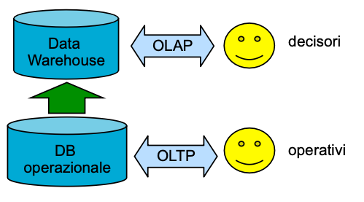
\includegraphics[width=0.7\linewidth]{img/DW}
	\caption{OLAP e OLTP}
	\label{fig:dw}
\end{figure}

Se riprendiamo l’esempio di FIAT, si nota che si ha un problema di prestazioni, perché si è cercato di lanciare una query OLAP sui database relazionali, che non sono progettati e ottimizzati per questo tipo di query. Come si può vedere dalla figura \ref{fig:dw} ho bisogno di separare l’elaborazione di tipo analitico (OLAP) da quella legata alle transazioni (OLTP), costruendo un nuovo repository di dati che è per l’appunto il \textbf{Data Warehouse}. Ho un’architettura con due DB separati: sotto tutti i DB operazionali con gli utenti OLTP che fanno ciò che facevano prima; sopra però creo un nuovo DB, in cui  si integrano tutti i dati che mi arrivano dalla sorgente di sotto, rendendoli disponibili ai decisori per l’analisi OLAP. Ho bisogno che tra i due mondi vi sia qualcuno che permette la sincronizzazione, e ciò è effettuato dall’\textbf{ETL (Extract Transform Load)}, ovvero una procedura batch, non interattiva, lanciata periodicamente per estrarre i nuovi dati che si sono cumulati nell’ultimo intervallo di tempo dalla fonte dei dati. L'ETL ha il compito di pulire i dati, di metterli in una forma diversa e di caricarli nel DW. Da evidenziare come nel DW le informazioni hanno sempre una certa latenza.

Con \textbf{Data Werahousing}, si fa riferimento al processo che estrae i dati e li trasforma in informazione, mentre con \textbf{Data Werahouse}, si fa riferimento al repository.

In particolare, il Data Werahousing è una collezione di metodi, tecnologie e strumenti di ausilio usati per permettere al knowledge worker di fare le sue analisi dei dati finalizzate all’attuazione di processi decisionali e al miglioramento del patrimonio informativo. 

Le \textbf{principali lamentele} sono:
\begin{enumerate}
	\item 
	Abbiamo montagne di dati ma non possiamo accedervi perché non conosco l’SQL per effettuare analisi
	\item 
	Come è possibile che persone che svolgono lo stesso ruolo presentino risultati sostanzialmente diversi?
	\item 
	Vogliamo selezionare, raggruppare e manipolare i dati in ogni modo possibile
	\item 
	Mostratemi solo ciò che è importante
	\item 
	Tutti sanno che alcuni dati non sono corretti
\end{enumerate}

La seconda e l’ultima sono quelle più importanti: spesso interrogazioni uguali forniscono risultati diversi e ancora più frequentemente nel DB sono inseriti dati sbagliati, o peggio ancora non sono proprio stati inseriti.
\subsection{Caratteristiche del processo di Data Warehosuing}
\begin{itemize}
	\item 
	\textbf{Accessibilità}: riferita ad utenti non ICT, non ho bisogno di essere un tecnico informatico, non devo conoscere strutture dati, SQL ecc.
	\item 
	\textbf{Integrazione dei dati}: devo avere una versione unica del dato
	\item 
	\textbf{Flessibilità di interrogazione}: dare all’utente un paradigma di interrogazione che sia non solo accessibile ma anche flessibile, ovvero permettere all’utente di lanciare query complesse mantenendo l’intuitività del programma applicativo
	\item 
	\textbf{Sintesi}: i dettagli inutili vengono scartati ma i dati vengono aggregati
	\item 
	\textbf{Rappresentazione multidimensionale}: le informazioni dentro al DW  vengono caricate in conformità al modello multidimensionale
	\item 
	\textbf{Correttezza e completezza}: pulitura dei dati
\end{itemize}
		\section{Il Data Werahouse}
Un \textbf{Data Warehouse} è una collezione di dati al supporto del processo decisionale con le seguenti caratteristiche:
\begin{itemize}
	\item
	È orientata ai soggetti di interesse (\textbf{subject oriented}): nasce per contrapposizione al mondo operazionale, in cui siamo application oriented. Infatti, quando si progettano database operazionali questi sono progettati finalizzati ad un’applicazione, quindi ad una macro-funzionalità. 
	\begin{figure}[H]
		\centering
		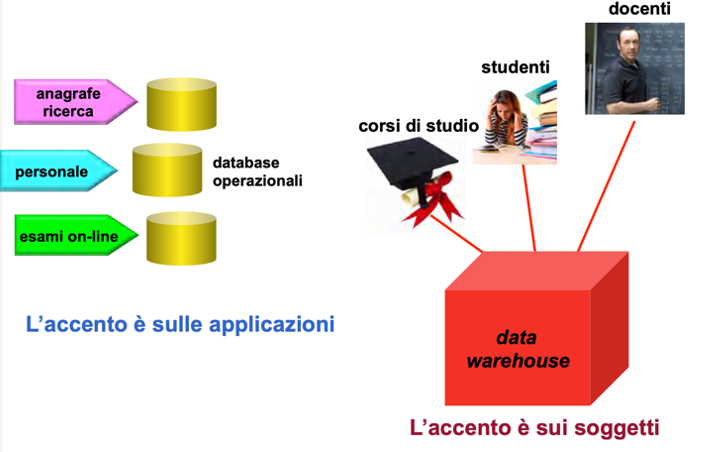
\includegraphics[width=0.7\linewidth]{img/SubjO}
		\caption{Subject Oriented}
		\label{fig:subjor}
	\end{figure}
	
	La conseguenza è che all’interno di ciascuno di questi database, di queste macro-funzionalità, i dati sono consistenti-integrati ma non lo sono rispetto ad altre funzionalità. Il senso di application oriented è che ogni applicazione è potenzialmente un mondo a sé. Quando si passa al contesto del DW, l’accento è sui soggetti, ovvero i protagonisti del business. A prescindere dalle funzionalità di ciascuno di questi soggetti io riesco a costruire dentro al DW una visiona completa in cui metto insieme tutto quello che quel soggetto fa o subisce. 
	\item 
	\textbf{È integrata e consistente}: è fondamentale che dentro al DW i dati che provengono dai diversi eterogenei database operazionali vengono combinati e riconciliati tra loro. Per prima cosa devo estrarre i dati, poi validare e pulire (eliminare per quando possibile gli errori), quindi li devo trasformare perché li devo integrare tra loro oltre che metterli in forma multidimensionale. Solo dopo posso caricarli nel data werahouse.
	Nei DB operazionali si può pensare che sia rappresentato in ogni istante una fotografia del business, i dati infatti sono soggetti ad aggiornamenti. Nel data werahouse buona parte delle query OLAP lavorano sui trend temporali. Ho bisogno di mantenere la storia, e immagino che l’ETL scatti una fotografia del business (DB operazionale) e la carica nel DW mettendola in coda a quelle precedenti. 
	\item 
	\textbf{È rappresentativa del tempo}
	\item 
	\textbf{Non volatile}: nel caso del DB operazionale il carico di lavoro OLTP è in lettura e in scrittura. Quindi in SQL, oltre alle SELECT, abbiamo INSERT, UPDATE e DELETE. Dentro al data werahouse, il carico di lavoro è in solo lettura. Ci sarà un momento in cui però andrò a scrivere, quando avvio l’ETL. In questo modo non ho problemi di accesso concorrenti in scrittura, e quindi non si pone il problema della transazione. L’unico problema che si ha è il query-throughput, cioè riuscire a dare buone prestazioni a diversi utenti che lanciano contemporaneamente delle query OLAP.
\end{itemize}
\begin{figure}
	\centering
	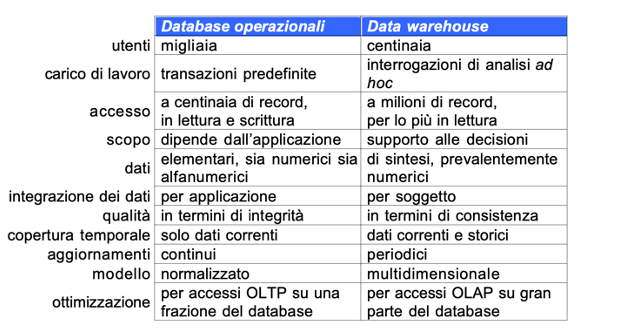
\includegraphics[width=0.9\linewidth]{img/DBeDW}
	\caption{Differenza DB operazionali e DW}
	\label{fig:differenze}
\end{figure}
\subsection{Architetture di Data Werahouse}
\subsubsection{I requisiti}
\begin{itemize}
	\item 
	\textbf{Separazione}: elaborazione analitica e quella transazionale devono essere mantenute il più possibile separate. 
	\item
	\textbf{Scalabilità}: con una crescita delle necessità, maggior volume dati e numero di utenti, si riesca a ridimensionare l’architettura HW-SW senza particolari problemi, non creando colli di bottiglia. 
	\item
	\textbf{Estendibilità}: poter aggiungere facilmente nuove applicazioni che interoperano con le precedenti
	\item
	\textbf{Sicurezza}: i dati che finiscono nel DW sono di importanza strategica per l’azienda; gli utenti del DW non possono vedere tutto ma accedono solo a porzioni più o meno ampie del DW
	\item
	\textbf{Amministrabilità}: la complessità dell’attività amministrativa non deve risultare troppo complesso da gestire
\end{itemize}
\subsubsection{Classificazione}

Una prima classificazione delle architetture è di tipo strutturale, in cui distinguiamo tre tipi di architetture in base al numero di livelli fisici presenti nell’architettura. 
La prima architettura, quella ad un livello, in figura \ref{fig:arch1} presenta un solo livello fisico, quello delle sorgenti in cui tengo traccia dei dati operazionali. Non si ha un DW fisico e in mezzo presenta un \textbf{middleware} (un sistema) che prende le query OLAP, le scrive sul DB operazionale, le esegue e restituisce i dati all’utente. Non rispetta il requisito della separazione.
\begin{figure}[H]
	\centering
	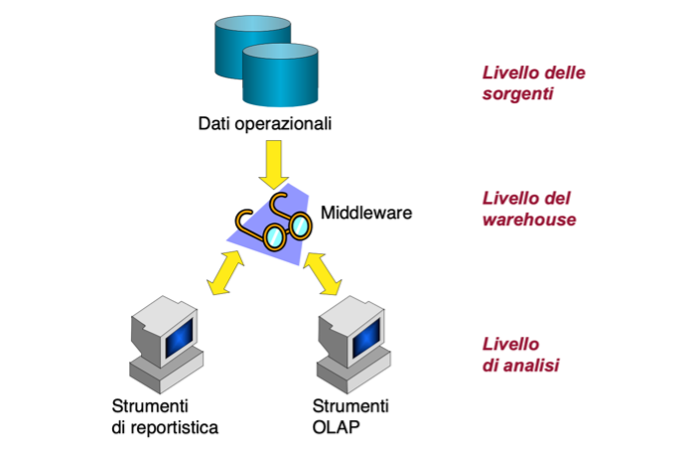
\includegraphics[width=0.6\linewidth]{img/arch1}
	\caption{Architettura ad un livello}
	\label{fig:arch1}
\end{figure}

L’architettura a due livelli presenta due livelli fisici, il livello della sorgente e il livello del werahouse e pertanto il requisito della separazione è soddisfatto. In mezzo c’è l’ETL che ha il compito di filtrare, estrare il distillato dei dati e caricarlo dentro al data werahouse. Dal livello di Dara Werahouse si accede al livello di analisi attraverso strumenti di reportistica, strumenti OLAP, analisi what-if ecc. I cilindri arancioni sono i data mart, ovvero porzioni di DW. Ciascun data mart è relativo ad una specifica area aziendale e quindi viene utilizzato da un sottoinsieme degli utenti. L’utilizzo dei data mart facilita il controllo degli accessi, perché il DW è già partizionato in data mart legati ad aree aziendali. Il data mart è l'incremento di progettazione e costruzione dei DW. Quindi questi vengono progettati e costruiti un data mart alla volta. 
\begin{figure}[H]
	\centering
	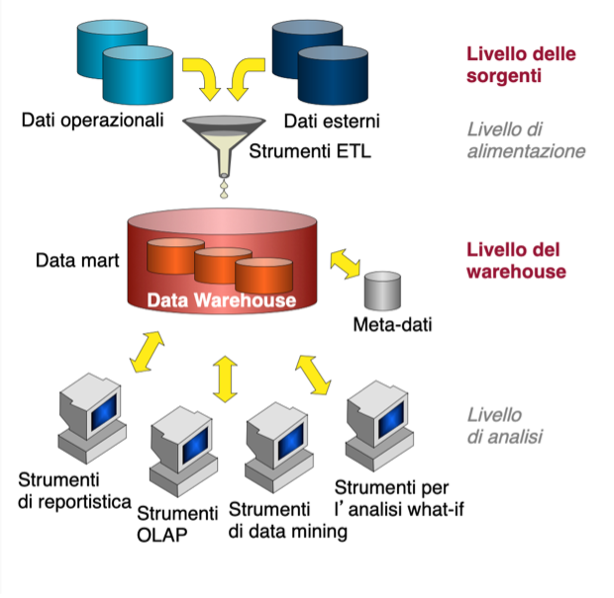
\includegraphics[width=0.6\linewidth]{img/arch2}
	\caption{Architettura a due livelli}
	\label{fig:arch2}
\end{figure}

L’architettura a tre livelli, in cui il nuovo livello fisico è quello dell’alimentazione, ovvero quello dell’ETL, la quale non viene vista solo come una procedura, ma ha il compito di “appoggiare” i risultati su un ulteriore DB, detto \textbf{ODS (Operation Data Store}). È un DB con dati operazionali, elementari, volatili, che si trovano a valle dell’ETL; quindi, sono dati puliti in quando gli errori sono stati già corretti. Successivamente vi è la fase di caricamento, i dati vengono estratti dall’ODS, messi in forma multidimensionale, aggregati per fare sintesi, e scritti dentro al DW. L'ODS assume un'importanza perchè questo è il luogo perfetto per lanciare la reportistica operativa. Infatti, nella piramide della BI, si nota che tra il livello inferiore dei dati e quello del data werahouse c’è proprio l’ODS. Cosa si intende per reportisca operativa? Un report è in generale, un risultato che si ottiene da una manipolazione dei dati. Il report strategico per i manager è di più alto livello; quindi, lavora con dati raggruppati (trend temporali ecc). Il report operativo è sempre una query in lettura, ma richiede un livello di dettaglio con solo dati correnti. Dunque, non serve ai livelli strategici ma ai livelli tattici. Spesso tali report non sono stati previsti nel momento in cui è stato progettato il DB relazionale, quindi non sono implementati. L’ODS è normalizzato, mentre il data werahouse no. \\

La seconda classificazione delle architetture  le distingue a seconda del modo con cui realizzano o non realizzano un’integrazione del dato a livello aziendale. Tali architetture sono:
\begin{itemize}
	\item 
	\textbf{Data mart indipendenti}: l’idea è che per ogni area aziendale ho fatto un progetto verticale senza tenere conto delle altre aree aziendali. Ho diversi data mart progettati indipendentemente gli uni dagli altri. In questo tipo di architettura i data mart vengono anche chiamati silos (compartimenti che non si parlano tra loro). Ad esempio voglio valutare un docente che tenga conto di quanti esami fa in un anno, di quanti articoli scrive, del suo ruolo, dello stipendio. Tutti questi numeri vengono da dati mart diversi, quindi per poter calcolare questo numero su ciascun docente ho bisogno di incrociare questi dati (JOIN). Il problema è che i data mart sono stati progettati separatamente e dunque il collegamento non è fattibile, perché ciascun data mart descrive il docente in maniera differente. L’architettura data mart indipendenti è veloce, relativamente economica, ma non è una buona architettura in quando non soddisfa il requisito di integrazione enterprise. 
	\begin{figure}[H]
		\centering
		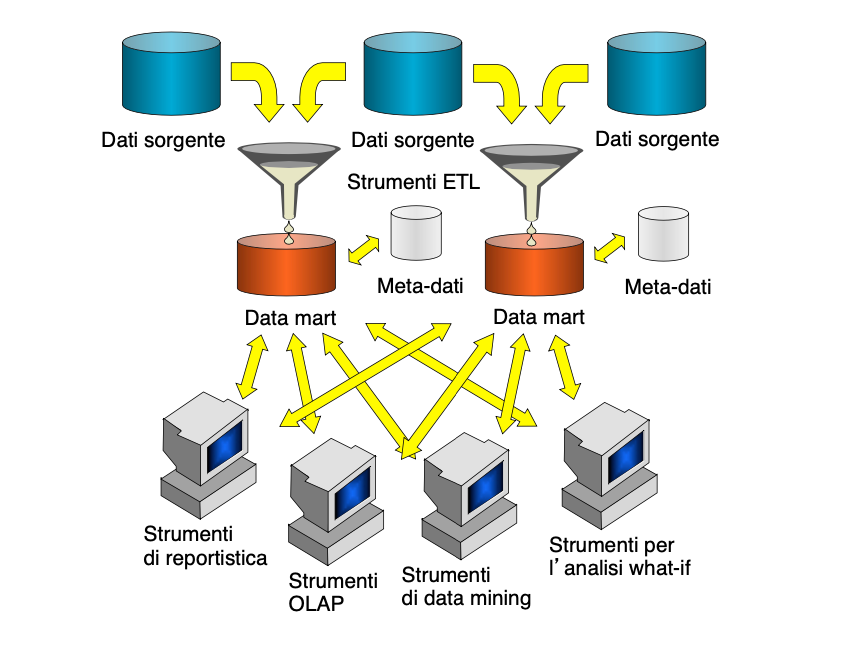
\includegraphics[width=0.5\linewidth]{img/DMind}
		\caption{Data Mart Indipendenti}
		\label{fig:dmind}
	\end{figure}
	\item 
	\textbf{Data mart bus}: simile all’architettura precedente con la differenza del blocco delle \textbf{dimensioni conforme}. Il trucco sta nel fatto che pur avendo dei mondi verticali si preveda all’inizio del progetto, un binario comune, che renda possibile l’integrazione dei data mart a posteriori. Quindi la enterprise view integrata del business la realizzo a livello logico. Le dimensioni conforme sono i concetti primari di business condivisi dalla maggior parte dei data mart. Prima di iniziare a realizzare il data mart prendo un cliente chiave da ciascuna area aziendale finché non si accordano su una definizione univoca sui diversi concetti chiave del business (dimensioni conforme). Dopo di che ogni reparto è libero di costruirsi il data mart come vuole ma con il vincolo di rispettare le dimensioni conformi. Il bello di questa architettura è che in ogni data mart posso decidere se usare un’architettura a due o tre livelli.
	\begin{figure}[H]
		\centering
		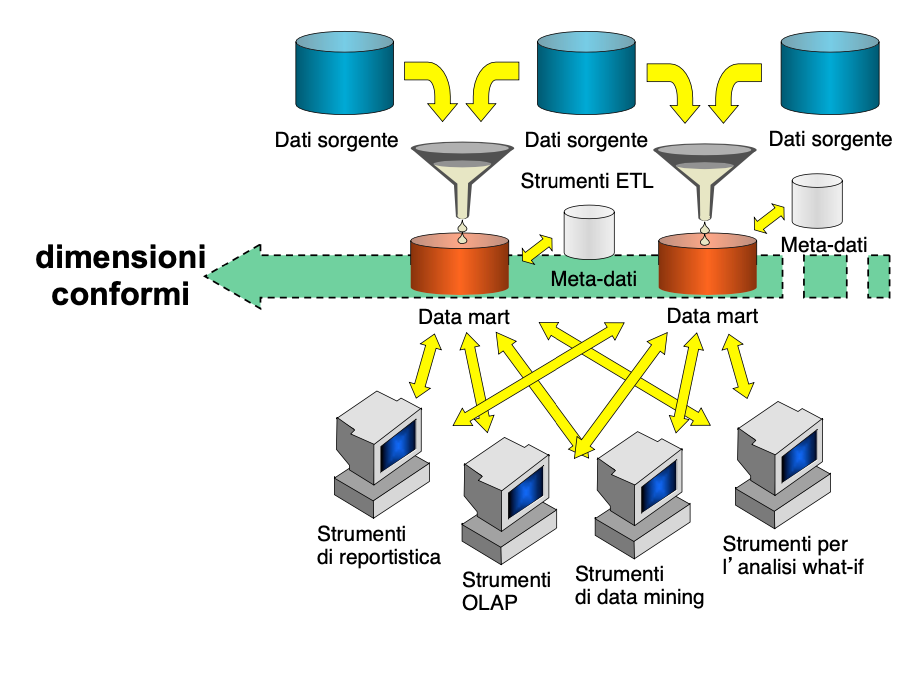
\includegraphics[width=0.5\linewidth]{img/DMcon}
		\caption{Data Mart Bus}
		\label{fig:dmbus}
	\end{figure}
	\item 
	\textbf{Hub-and-spoke}: questo tipo di architettura realizza nativamente un enterpise view. Per farlo utilizza un ODS enterprise \footnote{Un ODS a livello enterprise è relativamente complesso da progettare, perché bisogna mettere insieme idee e requisiti di tutti gli utenti aziendali e non solo ai principali soggetti del business} che copre tutta l’azienda, integrando tutti i dati aziendali, estraendo, solo dopo le singole informazioni per i vari data mart che sono allora volta integrabili. L’hub and spoke rispetto al data mart bus risulta essere più costoso.
	\begin{figure}[H]
		\centering
		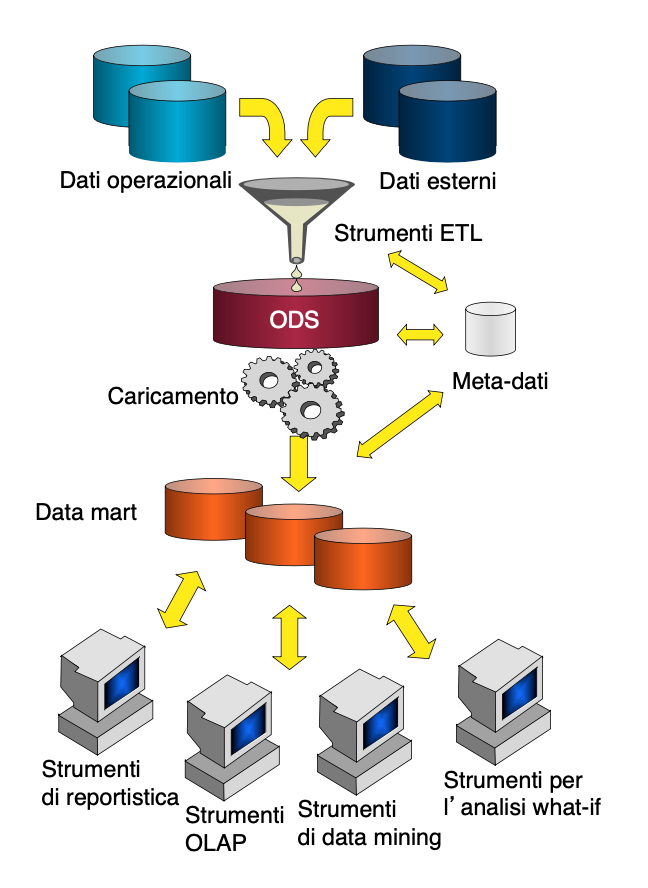
\includegraphics[width=0.2\linewidth]{img/hubandspoke}
		\caption{Hub and spoke}
		\label{fig:hubandspoke}
	\end{figure}
	\item 
	\textbf{Federazione}: il Data Werahouse federato si utilizza in due contesti: il primo è quello dinamico (fusioni-acquisizioni). L’esempio più eclatante è quello delle banche che uniscono rispettivamente i due business. Potrei mantenere entrambi i data werahouse ma prima o poi bisogna dare una versione unificata. Per fare ciò viene creato un DW di secondo livello. Grazie a ciò riesco ad incorporare nuovi DW senza doverli rifare da capo. L’architettura federata serve però anche come patch ad un’architettura data mart indipendente, progettando un DW di secondo livello, dove introducendo un livello di ETL ulteriore riesco a mettere insieme le cose. 
	\begin{figure}[H]
		\centering
		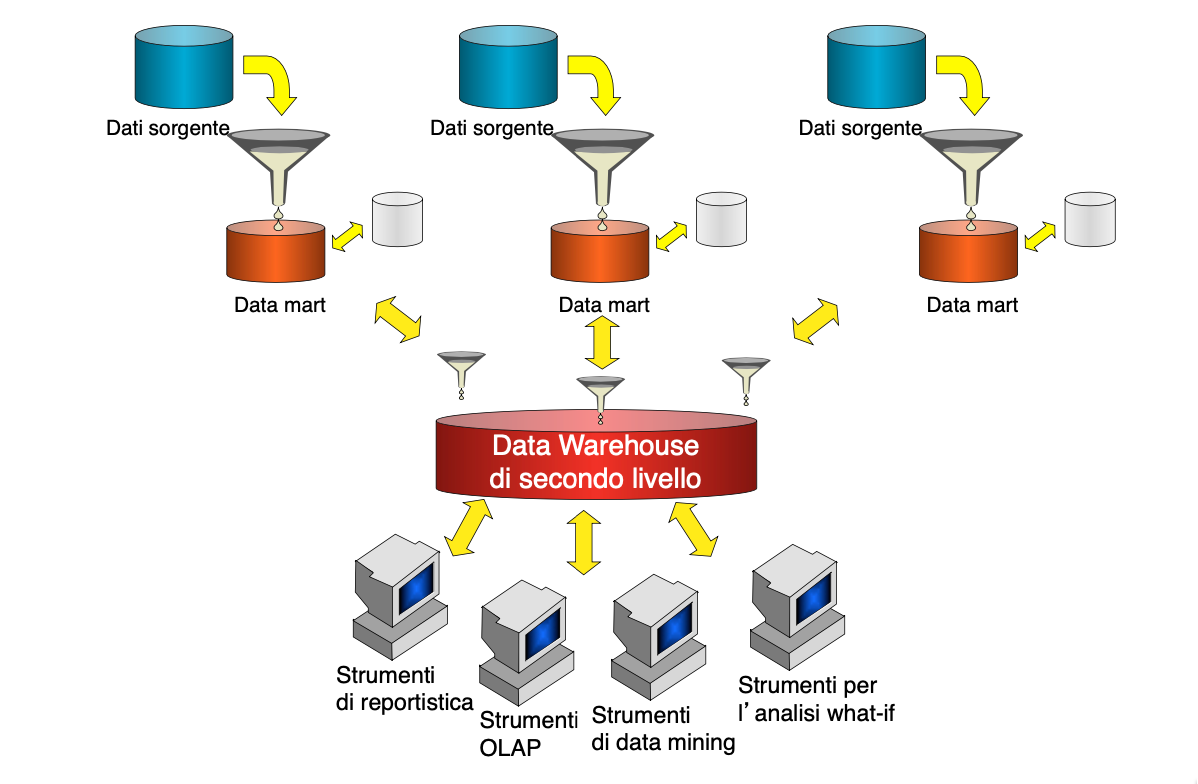
\includegraphics[width=0.7\linewidth]{img/fede}
		\caption{Federazione}
		\label{fig:federazione}
		
	\end{figure}
\end{itemize}
\subsubsection{Fattori di scelta dell'architettura}
La scelta dell’architettura dipende da diversi aspetti:
\begin{enumerate}
	\item 
	Bisogna capire quanto alta o bassa è la sponsorship del progetto, chi è che vuole il data werahouse? Il CEO o il mio capo reparto? Nel primo caso devo adottare un’architettura enterprise, nel secondo caso potrei optare per una data mart indipendente ma essere pronto al fatto che dovrò rimediare
	\item 
	Quanto le diverse unità organizzative in azienda sono legate tra di loro o meno (hub-and-spoke) o (data mart indipendent o bus)
	\item 
	Urgenza del progetto di data werahousing
	\item 
	Compatibilità con piattaforme esistenti: nei casi reali la software selection non si fa a 360 gradi, perché nella mia azienda ho già oracle o ibm e poiché sono orientato già verso uno stack tecnologico ho particolari vantaggi nel continuare a sposare quell’azienda.
\end{enumerate}
	\section{ETL}

Questi strumenti hanno un ruolo fondamentale nell’architettura di DW perché innanzitutto sono garanti delle qualità e poi perché sono quelli che popolano il data werahouse. L’ETL in presenza di un database riconciliato, quindi di un ODS, avviene in due step.Il primo si occupa di estrarre dal database sorgente, trasformare e caricare sull’ODS. Il secondo, invece, si occupa di prendere i dati dall’ODS e metterli sul data mart. Evidentemente ci sono due modalità per lanciare l’ETL. La prima è quella che si lancia quando il sistema di DW entra in produzione,ovvero quando viene popolato con informazioni per la prima volta. L’altra modalità avviene periodicamente. 

L’ETL può essere implementato in due modi: lo si può scrivere come se fosse una procedura o lo si può realizzare usando uno strumento commerciale. Nel primo caso il vantaggio è avere un controllo perfetto su quello che sta succedendo e su come gestisco la procedura. Tale metodo è lungo e complesso da scrivere ed è altrettanto complesso da documentare e mantenere. Utilizzare gli strumenti commerciali permette di avere un ambiente, al cui interno, in modalità grafica posso disegnare i flussi per l’ETL. Tutto questo per ottenere tempi ridotti per la costruzione dell’ETL e un minor sforzo per fare la documentazione. In ogni caso le query, o le procedure di pulizia vanno comunque scritte. Un buon ETL vuol dire aver trovato la maggior parte degli errori e correggerne qualcuno. Non sempre però è possibile correggere in automatico gli errori. 
\subsection{Estrazione}
Bisogna estrarre dalle sorgenti dati tutto ciò che serve per essere rielaborato e aggiunto dentro al DW. L’estrazione può essere fatta in due modi:
\begin{itemize}
	\item 
	\textbf{Estrazione statica}: viene effettuata quando il DW deve essere popolato per la prima volta e consiste in una fotografia dei dati operazionali
	\item 
	\textbf{Estrazione incrementale}: l’idea è quella di estrarre dal database sorgente solo quello che è cambiato rispetto all’ultima estrazione. L’estrazione incrementale ha qualche complessità in più rispetto all’estrazione statica. 
\end{itemize}
\subsection{Pulitura}
Si intende tutte le modifiche che si fanno al valore dei dati con l’obiettivo di correggere gli errori e quindi migliorare la qualità del dato. Esistono errori di diversa natura, in molti casi, legati ad un insufficiente controllo di input:
\begin{itemize}
	\item
	\textbf{Dati duplicati}: per certi pazienti mi ritrovo più record distinti. Inconsistenza tra valori logicamente associati
	\item
	\textbf{Dati mancanti}: chi compila un’anagrafica richiede solo i dati obbligatori; quindi, successivamente mi ritrovo dei NULL
	\item
	\textbf{Uso non previsto di un campo}: campi di tipo note o commenti dove un utente potrebbe scrivere dei dati che sono importanti per il processo decisionale
	\item
	\textbf{Valori impossibili o errati}: esempio nome di un comune che non esiste
	\item 	
	\textbf{Valori inconsistenti per la stessa entità dovuti a errori di battitura}: utente che compare in due database ma con codice fiscale differente
\end{itemize}
\subsection{Trasformazione}
Lavora sul formato dei dati, con l’obiettivo di riportare tutti i dati ad un unico standard di rappresentazione. Per poter riconciliare i database bisogna imporre un unico standard. La trasformazione viene fatta a valle e a monte dell’ODS. A monte, sui dati estratti dai DB operazionali per poi caricarli sull’ODS. Quello che si deve fare è standardizzare, normalizzare, matching e selezione, perché magari certi campi non sono d’interesse per il DW. L’altra parte di ETL prevede una denormalizzazione e l’introduzione di aggregazione, eliminando magari il dettaglio più fine di granularità del dato che non sia importante per il processo di supporto decisionale, quindi effettuando sintesi. (esempio slide pag. 36)
\subsection{Caricamento}
Simmetricamente a quello fatto in estrazione, il caricamento dei dati lo posso fare in due modi:
\begin{itemize}
	\item 
	\textbf{Refresh}: riscrivo tutto 
	\item 
	\textbf{Update}: aggiungo la nuova fotografia a quelle precedenti, aggiungendo una nuova fetta di dati
\end{itemize}
	\section{Il modello multidimensionale}

È il modello utilizzato per la rappresentazione delle informazioni all’interno dei data mart. Si è scelto questo modello perché molto intuitivo ed è già alla base del foglio elettronico che i manager sono abituati ad utilizzare. L’altro motivo per cui è stato  scelto è che larga parte delle query OLAP sono facilmente formulabili proprio in riferimento al modello multidimensionale. Il punto fondamentale è il concetto di \textbf{fatto}, ovvero un fenomeno di business che accade dinamicamente nell’azienda e che gli utenti sono interessati a monitorare (vendita, spedizione, fattura). In una prima presentazione del modello multidimensionale si usa una metafora che è quella del cubo, fatto da tante celle e costituito da tre spigoli, che rappresentano le dimensioni, ovvero attributi che sono utilizzati per selezionare e aggregare le celle dei cubi. Dentro ad una cella vi è un numero, che noi chiamiamo \textbf{misura}, il quale quantifica il fatto da un certo punto di vista. 
\begin{figure}[H]
	\centering
	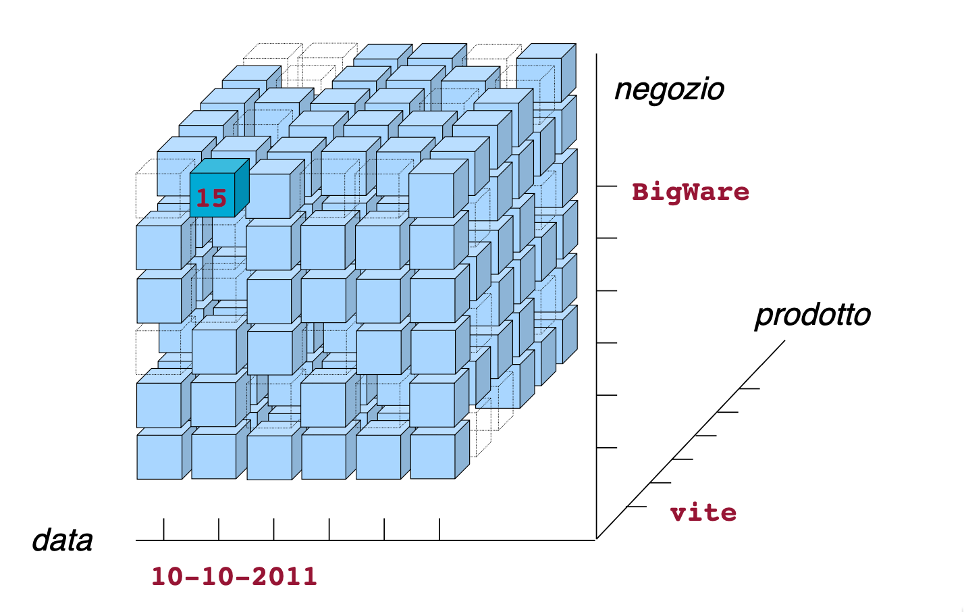
\includegraphics[width=0.7\linewidth]{img/example}
	\caption{Esempio modello multidimensionale}
	\label{fig:model}
\end{figure}
Nell'esempio in figura \ref{fig:model} sto dicendo che in quella data, nel negozio BigWare, ho venduto 15 viti. Supponendo di avere le seguenti cardinalità:
\begin{itemize}
	\item 
	Negozio : $10^{3}$
	\item 
	Data: $10^{3}$
	\item 
	Prodotto: $10^{4}$
\end{itemize}
La cardinalità massima del cubo se non ci fosse sparsità sarebbe $10^{10}$. Supponendo che un prodotto ogni 10 in un negozio e per ciascuna data resti invenduto, la cardinalità reale sarebbe di $10^{9}$. \\

Ho bisogno di tecniche per riuscire ad analizzare le informazioni in maniera più agevole, in moda da ridurne ulteriormente la mole. Nel modello multidimensionale ho due tecniche: \textbf{selezione} e \textbf{aggregazione}. L’idea della selezione, al momento del lancio di una query OLAP, è quella di concentrarsi su alcuni dati e non su altri. Nel modello multidimensionale esistono due modi differenti per fare selezione: \textbf{slicing} e \textbf{dicing}. Fare slicing significa focalizzarsi su una fetta di dati. Per fare ciò io fisso un valore da una dimensione e seleziono le celle corrispondenti a quel valore. Con il dicing io seleziono un sotto cubo rispetto al cubo di partenza specificando degli intervalli. 
\begin{figure}[H]
	\centering
	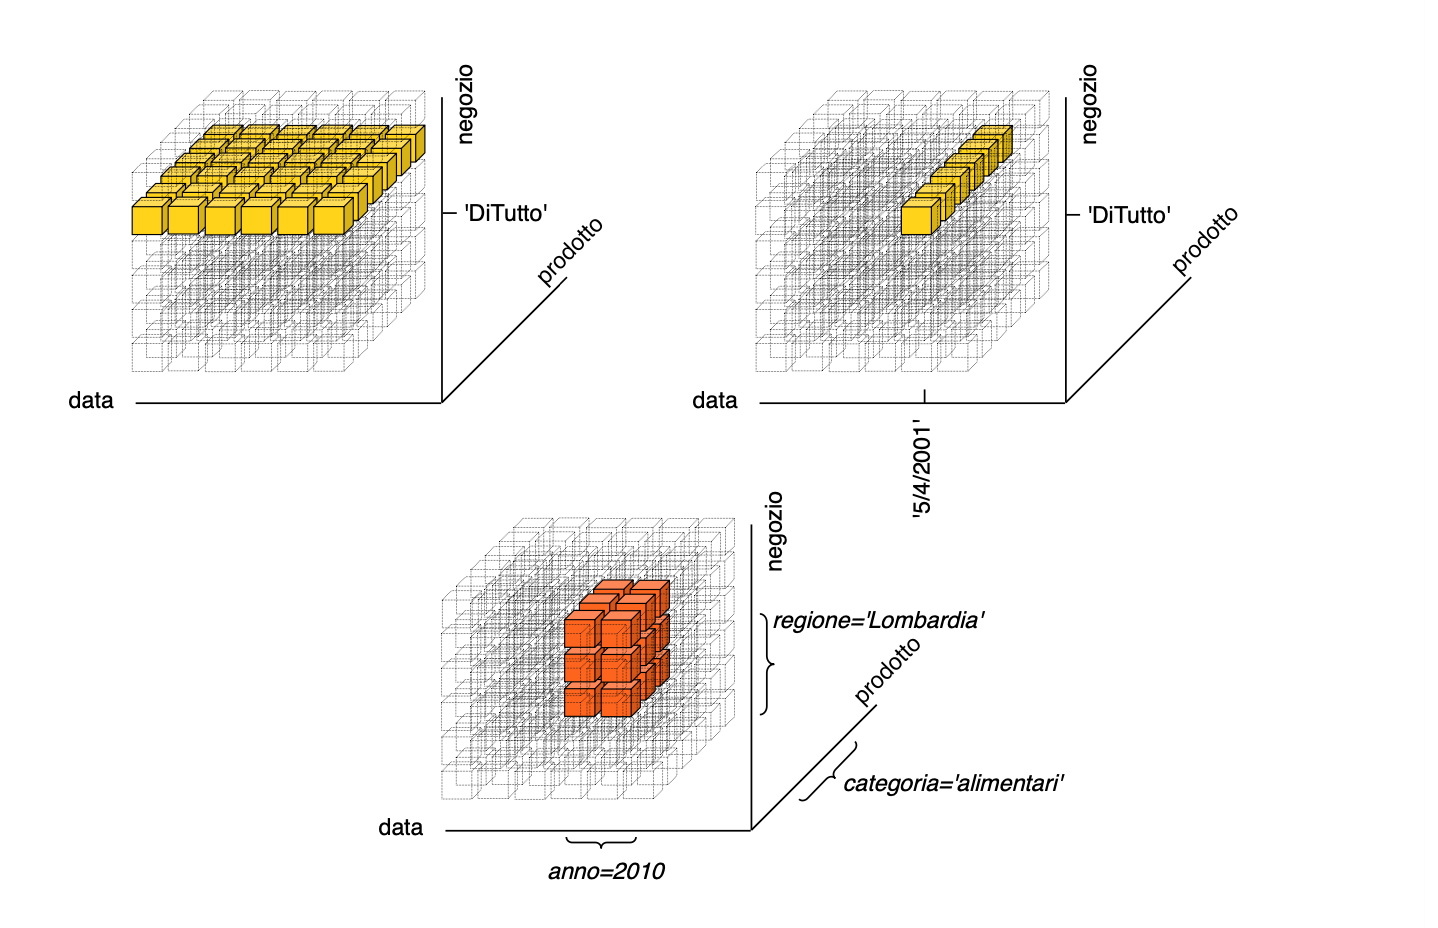
\includegraphics[width=0.5\linewidth]{img/slicing&dicing}
	\caption{Slicing and dicing}
	\label{fig:slice}
\end{figure}

Per introdurre l’\textbf{aggregazione} bisogna aggiungere il concetto di gerarchia. Una \textbf{gerarchia} è una sequenza di attributi che parte da una dimensione, nel nostro caso prodotto e negozio, collegati tra di loro da associazioni molti ad uno. 

Dato il cubo delle vendite, potrei come utente decidere che questo livello di dettaglio è troppo e vorrei analizzare il fenomeno ad un livello di granularità meno fine.
\begin{figure}[H]
	\centering
	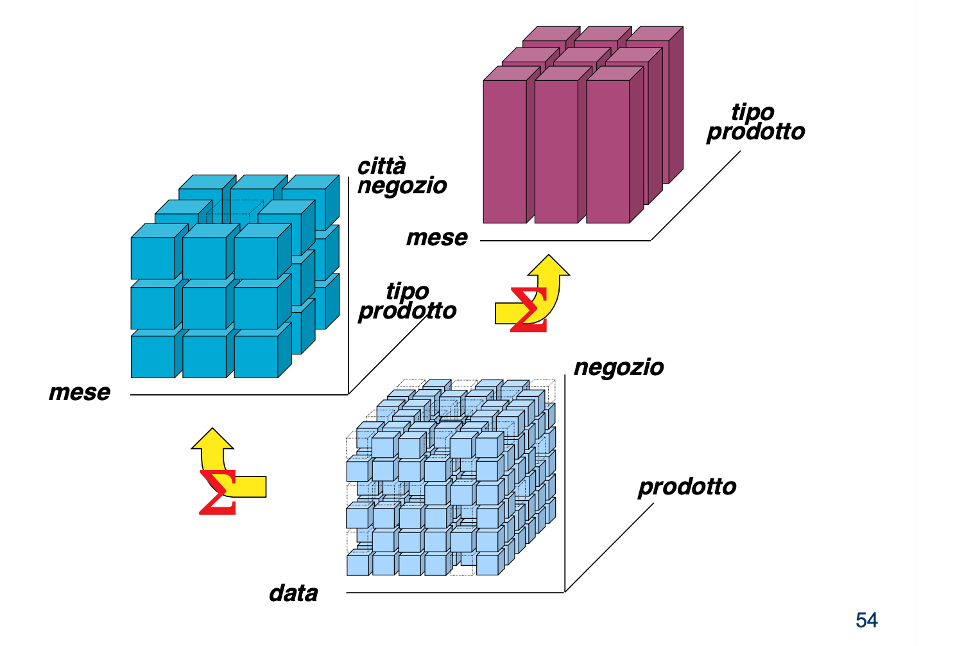
\includegraphics[width=0.6\linewidth]{img/gran}
	\caption{Aggregazione}
	\label{fig:aggregazione}
\end{figure}
\subsection{Analisi dei dati}
Esistono due approcci differenti, supportati da altrettante categorie di strumenti, all’interrogazione di un DW da parte degli utenti finali:
\begin{itemize}
	\item 
	\textbf{Reportistica}: non richiede conoscenze informatiche. La reportistica viene chiamata anche reportistica statica, per evidenziare il fatto, che quando si fa reportistica l’utente ha un ruolo passivo perché i report vengono decisi al momento del progetto e non sono modificabili interattivamente dagli utenti. Nel caso della reportistica si lavora come nel caso dell’OLTP congelando le query frequenti dentro la logica applicativa. 
	\item
	\textbf{OLAP}: ho bisogno di conoscere l’interfaccia dello strumento grafico utilizzato e avere chiaro il modello multidimensionale. Nel caso dell’OLAP l’utente non ha più un ruolo passivo ma attivo, perché sceglie quale query formulare. Gli utenti OLAP sono in grado di costruire attivamente una sessione di analisi, cioè dei percorsi di esplorazione all’interno del cubo. In questo modo pur non essendo un esperto di informatica, riesce a costruire delle sessioni di lavoro estemporanee, formulando anche delle query complesse. Una \textbf{sessione} è una sequenza di query formulate per differenza rispetto alle precedenti. Ogni passo della sessione è scandito dall’applicazione di un operatore OLAP che trasforma l’ultima interrogazione formulata in una nuova interrogazione. Il risultato delle interrogazioni è di tipo multidimensionale. 
\end{itemize}
\subsubsection{Gli operatori OLAP}
\begin{itemize}
	\item
	\textbf{Roll-Up}: parte da una certa situazione di analisi di dettaglio e  porta a fare uno zoom-out, cioè permette di aggregare il cubo. 
	\item 
	\textbf{Drill-down}: parte da un cubo grossolano e fa uno zoom-in, cioè si avvicina e scorpora i dati nelle sue componenti. Nel fare questo può anche iniettare in un cubo una dimensione che prima non c’era. 
	\item 
	\textbf{Slice-and-dice}: è un operatore di selezione che permette di focalizzarsi su un sottoinsieme di eventi del fatto o attraverso uno slicing o attraverso un dicing. La differenza è di tipo concettuale perché l’operatore è unico. 
	\item 
	\textbf{Pivoting}: è un operatore che cambia il modo per visualizzare i dati, inverte righe e colonne.
	\item 
	\textbf{Drill-across}: è un operatore di sostanza e permette di stabilire una corrispondenza tra due cubi distinti. Mette in corrispondenza una cella di un cubo con un’altra cella dell’altro cubo. Serve quando bisogna valutare una misura che ottengo applicando una formula a misure che stanno su cubi diversi. 
	\item 
	\textbf{Reportistica semi-statica}: è un approccio intermedio tra reportistica statica e OLAP. La reportistica semi-statica nasce per evitare che un cliente malaccorto lanci delle query troppo dettagliate che possano piantare il DW o aggregare con diversi operatori, ottenendo strani risultati. Si immagini che la reportistica semi-statica sia un prato in cui ci si possa muovere in alcune direzioni e non in altre; quindi, dove comunque ho dei percorsi di aggregazione.
\end{itemize}
\subsection{Implementazione Data Werahouse}
Esistono tipicamente due piattaforme tecnologiche per l’implementazione del DW:
\begin{itemize}
	\item 
	\textbf{ROLAP (Relational OLAP)}: è un’implementazione relazionale e dunque il dato multidimensionale alla fine viene implementato su un server relazionale (tabelle). Perché usare un DB relazionale se ho un modello diverso? I database relazionali sono diffusi in azienda e quindi si cerca di utilizzare ciò anche nell’ambito del DW. Devo affrontare il problema del miss match, cioè la mancata corrispondenza tra i due modelli, perché l’utente ragionerà in termini di cubi ma sotto ho delle relazioni. Per saltare questo passaggio bisogna usare delle forme particolare dei modelli relazionali per ospitare dati multidimensionali (schema a stella). Ho un problema di traduzione che viene effettuata nei due versi da un componente detto motore multidimensionale, il quale si appoggia a dei metadati per restituire una visione multidimensionale di dati relazionali. 
	\begin{figure}[H]
		\centering
		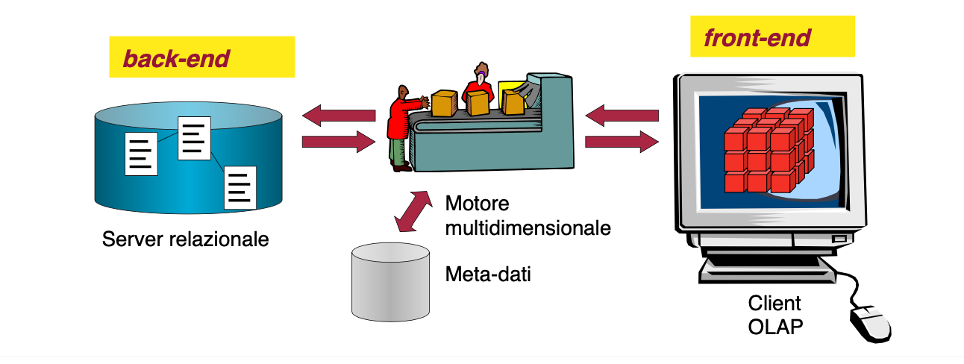
\includegraphics[width=0.7\linewidth]{img/rolap}
		\caption{ROLAP}
		\label{fig:rolap}
	\end{figure}
	Mi aspetterei potenziali problemi di prestazioni, perché per lavorare sui DB relazionali, ho bisogno di fare join che sono operazioni costose tanto più fatte su tabelle che hanno milioni di righe. Si utilizzano tecniche particolare per evitare questi problemi, come la denormalizzazione.
	\item 
	\textbf{MOLAP (Multidimensional OLAP}): basato su un database che è nativamente multidimensionale, costruito ad hoc, i dati sono allocati dentro una matrice ad accesso posizionale. Le prestazioni risultano essere ottime perché non ho bisogno di join ma al contempo ho il problema della sparsità, perché mentre in una tecnologia ROLAP nelle tabelle ho righe solo per gli eventi che si verificano, in MOLAP devo allocare tutto il cubo. Ogni piattaforma MOLAP utilizza un suo metodo per gestire la sparsità e sono poco utilizzati. 
	\item 
	\textbf{HOLAP (Hybrid OLAP)}: combinazione tra le due tecnologie in cui tipicamente i dati di dettaglio sono memorizzati su DBMS relazionale, i pre-aggregati su strutture multidimensionali proprietarie. Oppure, i sotto cubi densi sono memorizzati in forma multidimensionale, quelli sparsi in forma relazionale. 
\end{itemize}
\subsection{Qualità e Sicurezza}
In termini generali la qualità di un processo misura la sua aderenza agli obiettivi degli utenti. Nella fattispecie quando si parla di DW interessa la qualità dei dati, il quale è legata ad una buona realizzazione dell’ETL. La qualità dei dati all’interno del DW ha diversi aspetti:
\begin{itemize}
	\item 
	\textbf{Accuratezza}: c’è conformità tra il valore memorizzato e quello reale
	\item 
	\textbf{Attualità}: il dato è attuale e non obsoleto (dipende dalla frequenza dell’ETL)
	\item 
	\textbf{Completezza}: non mancano informazioni
	\item 
	\textbf{Consistenza}: sono effettivamente riuscito a superare l’eterogeneità dei dati
	\item 
	\textbf{Disponibilità}: i dati sono facilmente disponibili all’utente
	\item
	\textbf{Tracciabilità}: è possibile risalire alla fonte di ciascun dato, stabilire un collegamento tra il DB del data werahouse e il DB operazionale, in cui trovo i singoli documenti
	\item 
	\textbf{Chiarezza}: i dati sono facilmente interpretabili
\end{itemize}
Quando un progetto di DW va a regime, cioè entra in produzione,  occorre necessariamente che l’azienda attui un processo di certificazione, ossia deve individuare delle persone che siano responsabili del dato. È chiaro che questo sia un ruolo di business e non informatico, che ha dunque la sensibilità del dato. In assenza di certificazione non ho nessuna garanzia sulla qualità. 

All’interno del DW ci finiscono informazioni che sono assolutamente strategiche e che quindi non devono finire in mano ai competitor o a certi ruoli aziendali. Spesso nei DW si attua una compartimentazione dell’informazione. Ogni capo reparto vede i dati solo del suo reparto. La \textbf{sicurezza} in primis viene implementata attraverso un controllo molto stretto delle autorizzazioni, che si svolge in genere sugli strumenti di front-end OLAP. Si utilizzano meccanismi di auditing per monitorare gli accessi, il che risulta più complicato, perché siamo in presenza di aggregazione. 
		\section{Il ciclo di vita del Data Warehouse}
Trattandosi di sistemi complessi è fondamentale seguire una metodologia. Questi progetti hanno diversi fattori di rischio:
\begin{itemize}
	\item
	Rischi legati alla gestione del progetto
	\item 
	Rischi legati alle tecnologie
	\item 
	Rischi legati ai dati e alla progettazione
	\item 
	Rischi legati all'organizzazione
\end{itemize}
Esistono due macro-approcci di progettazione:
\begin{itemize}
	\item 
	\textbf{Top-down}: significa pensare, concepire, progettare e costruire il DW come un monolite, cioè considerando i bisogni di tutta l’azienda in modo da coprirli per intero. In linea di principio, questo è un metodo eccezionale, perché si basa su una visione globale e garantisce di ottenere una perfetta integrazione consistente tra i reparti. Questo comporta fare un’analisi con tutti gli utenti dell’azienda e  capire come sono fatti tutti i DB aziendali. Questo può portarmi alla paralisi dell’analisi, cioè  arrivare in una situazione in cui il costo dell’analisi diventa eccessivo. Inoltre, è difficile prevedere a priori le esigenze di tutti gli utenti. Il fatto di non prevedere una consegna a breve termine non permette agli utenti di verificare l’utilità del progetto e ne fa scemare l’interesse e la fiducia. 
	\item 
	\textbf{Bottom-up}: costruire il DW in modo incrementale, un pezzo alla volta. Solo alla fine ho la visione globale del DW. Il pezzo utilizzato nel metodo incrementale è proprio il data mart. L’idea di questo approccio è pensare, progettare ed implementare un data mart alla volta. Ciò determina risultati concreti in tempi brevi. Il progettista deve fare analisi dei requisiti solo su un ‘area aziendale e per alimentare quel data mart non ho bisogno di tutti i DB aziendali, ma solo di qualcuno. Altro vantaggio è quello di mantenere elevato l’attenzione degli utenti sul progetto.
\end{itemize}

Il primo passo per la realizzazione di un DW è scegliere il primo data mart, il quale deve essere strategico, cioè coprire un ruolo centrale e di riferimento per l’intero DW. Si deve appoggiare su fonti dati già disponibili e consistenti. 

A livello macroscopico il ciclo di sviluppo può essere rappresentato dalla figura \ref{fig:ciclo}. 
\begin{figure}[H]
	\centering
	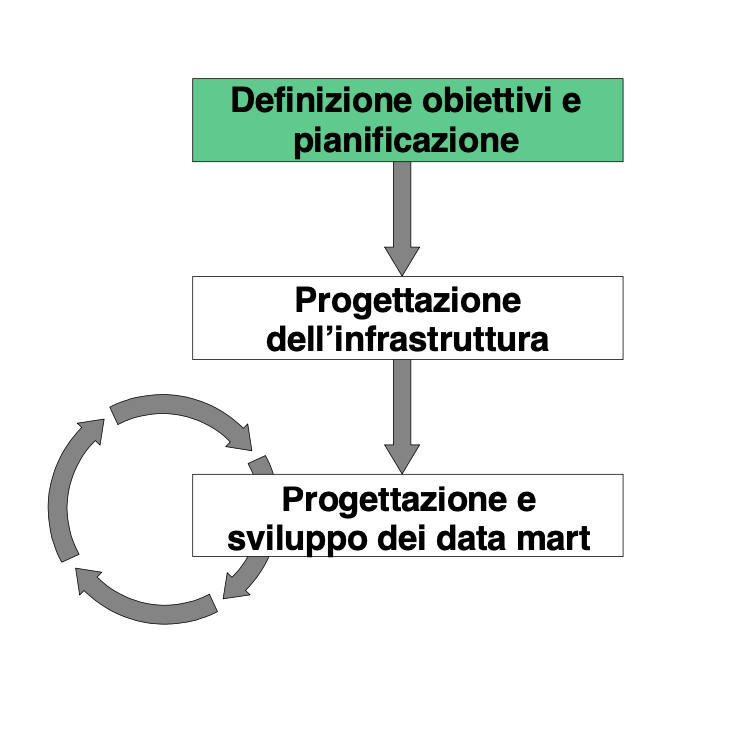
\includegraphics[width=0.5\linewidth]{img/cicloDW}
	\caption{Ciclo DW}
	\label{fig:ciclo}
\end{figure}
Vi è una prima di fase di definizione degli obiettivi e dei confini, in cui si prepara una roadmap di progetto per il medio lungo termine. Questa fase comporta la scelta dell’architettura. 

La seconda fase è di progettazione dell’infrastruttura e prevede la scelta dello stack tecnologico. Molte volte questa scelta non risulta essere libera perché ci si basa sulle tecnologie che già si hanno in casa e anche per avere meno problemi di interoperabilità tra i software. 

L’ultima fase è la fase iterativa, in cui ad ogni giro, si realizza un nuovo data mart che viene integrato nel sistema di DW. 
\subsection{Progettazione del data mart}
La progettazione di data mart coinvolge diverse figure, quali il progettista, l’amministratore di db e l’utente finale, ed è composta da diverse fasi:
\begin{itemize}
	\item
	\textbf{Analisi e riconciliazione delle sorgenti}: l’idea è capire come sono fatte le basi di dati utilizzate come sorgenti per alimentare il data mart. Le sorgenti dati sono analizzate, normalizzate e integrate per ottenere uno schema riconciliato per l’ODS
	\item 
	\textbf{Analisi dei requisiti}: capire che cosa gli utenti devono fare con questo sistema, cioè quali fatti devono modellare, con quali dimensioni, con quali misure, in modo da ottenere report e risultati di analisi. Questa fase avviene attraverso delle interviste
	\item
	\textbf{Progettazione concettuale}: rappresenta i concetti che devono essere gestiti nel DB in maniera indipendente dall’implementazione. In questo caso significa disegnare uno schema concettuale del data mart, cioè uno schema che spiega il contenuto informativo ma senza entrare nel merito dell’implementazione. Lo schema concettuale per essere corretto dovrà tener conto dei dati sorgenti e rispettare i requisiti utente. 
	\item 
	\textbf{Carico di lavoro e volume dati}: insieme delle query che verranno sottoposte al sistema. Si profilano gli utenti (coordinatore corso di studi, preside ecc.) e infine si misura il volume dati.
	\item 
	\textbf{Progettazione logica}: riprendo lo schema concettuale e lo traduco in uno schema logico, il che è dipendente dall’implementazione, in cui scelgo il tipo di piattaforma implementativa (ROLAP o MOLAP). 
	\item 
	\textbf{Progettazione dell’ETL}: si progettano le procedure ETL, le quali come abbiamo già detto, hanno il compito di “rinfrescare” i contenuti del data mart tenendo conto delle modifiche fatte nel DB sorgente.
	\item
	\textbf{Progettazione fisica}: non mi basta aver scelto l’implementazione, ma devo sapere anche qual è lo stack tecnologico. Devo tipicamente creare gli indici, e poiché ogni specifico DBMS ha le sue regole, in questa fase devo sapere su quale stack tecnologico mi devo muovere.
	\item 
	\textbf{Implementazione della reportistica}: si creano i report a partire dal carico di lavoro. Resto sul front-end che ho scelto, creo i meta dati e devo creare i report. 
	\item 
	\textbf{Testing}: si testano le procedure ETL e i report
\end{itemize}
Le diverse fasi possono incastrarsi in maniera diversa e a seconda del quadro metodologico che adotto:
\begin{itemize}
	\item 
	\textbf{Approccio guidato dai dati (supply-driven)}: la forma dei DB sorgente mi guida nella progettazione del data mart. I requisiti utente impattano sul progetto guidando il progettista nella selezione delle porzioni di dati considerate rilevanti per il processo decisionale, e determinando la loro strutturazione secondo il modello multidimensionale
	\item 
	\textbf{Approccio guidata dai requisiti (demand-driven)}: quello che mi traina nella progettazione sono i requisiti dell’utente
\end{itemize}
\subsubsection{Supply-Driven}
Come riportato in figura \ref{fig:supply} inizio con il guardare il contenuto delle sorgenti. Le sorgenti sono caratterizzate attraverso i loro schemi. Nel caso di DB relazionale ho lo schema logico o un entity-relation. L’analisi e la riconciliazione nello specifico prevede l’integrazione degli schemi in modo da avere in uscita uno schema riconciliato, che mi restituisce una visione unica di quella fetta di dato. In un’architettura a tre livelli, quello schema diventa lo schema dell’ODS. Quindi effettuo l’analisi dei requisiti
attraverso le interviste e in un’uscita si possono usare dei glossari tenendo traccia delle cose principali che mi hanno detto gli utenti. Quindi posso passare alla progettazione concettuale, prendendo lo schema riconciliato e ottenendo uno schema per i data mart, detto schema di fatto. Intanto lavoro sul carico di lavoro e volume dati, scrivendomi le query più frequenti e la reportistica che potrebbe servire. Adesso si è pronti per fare la progettazione logica, si prende lo schema di fatto e tenendo conto di carico e lavoro di volume dati, lo si traduce in uno schema logico. A questo punto posso passare alla progettazione dell’ETL e infine alla progettazione fisica, scegliendo il DBMS e ottenendo dallo schema logico lo schema fisico. 
\begin{figure}[H]
	\centering
	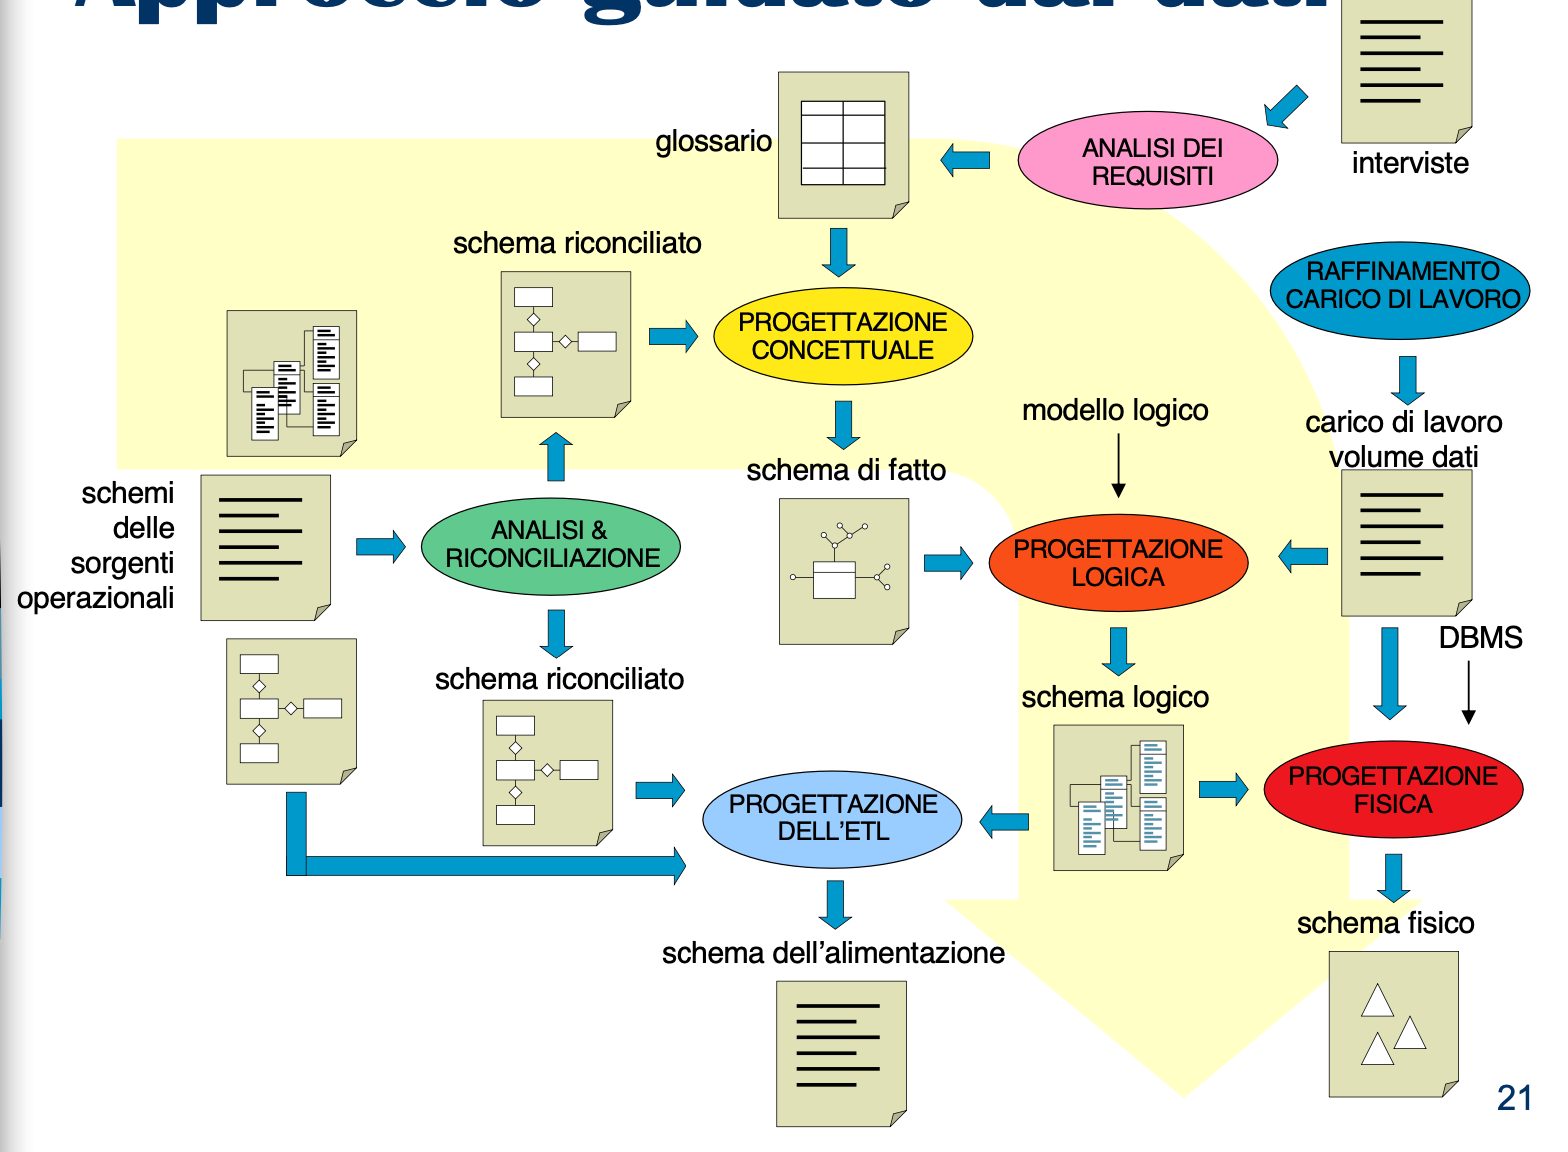
\includegraphics[width=0.7\linewidth]{img/supply-driven}
	\caption{Supply-Driven}
	\label{fig:supply}
\end{figure}
\textbf{Vantaggi}

Il grosso vantaggio è l’esistenza di un algoritmo che banalizza la fase di progettazione concettuale a partire dai dati riconciliati. 

L’algoritmo come prodotto laterale restituisce i mapping tra i concetti del data mart e i concetti dello schema sorgente. 

\textbf{Svantaggi}

Ai requisiti utente viene assegnato un ruolo secondario nel determinare i contenuti informativi per l’analisi, mentre al progettista viene dato un supporto limitato per l’identificazione di fatti, dimensioni e misure.

\textbf{Applicabilità}

Tale approccio è applicabile quando:
\begin{itemize}
	\item 
	Conosca in anticipo gli schermi delle sorgenti e questi siano normalizzati e non complessi, perché quest’algoritmo si nutre di dipendenze funzionali, cioè funziona andando a leggere le dipendenze funzionali codificate nel DB sorgente
	\item 
	Quando l’architettura prescelta prevede l’adozione di un livello riconciliato questi requisiti sono soddisfatti: la normalizzazione e la conoscenza approfondita sono garantite dalla riconciliazione. Lo stesso vale nel caso in cui la sorgente si riduca ad un singolo Database, ben progettato e di dimensioni limitate
	\item
	Risulta essere l’approccio preferibile perché meno soggetto a errori ed estremamente più veloce del demand-driven.
\end{itemize}

\subsubsection{Demand-Driven}
Nel secondo tipo di approccio si parte dall’analisi dai requisiti e sulla base dei requisiti utente disegno lo schema concettuale. Una volta effettuata anche la fase del carico di lavoro posso passare alla progettazione logica, in modo da creare lo schema del DB del data mart sulla base dei requisiti utente. Passo alla progettazione dell’ETL partendo dagli schemi sorgenti, ma adesso questo risulta essere più costoso. Infine, passo alla progettazione fisica.\\

\textbf{Vantaggi}

I desideri degli utenti vengono portati in primo piano

\textbf{Svantaggi}

È richiesto al progettista uno sforzo consistente durante il disegno dell’alimentazione. Dunque fatti, misure e gerarchie vengono ricavate direttamente dalle specifiche dettate dagli utenti, e solo a posteriori si verifica che le informazioni richieste siano effettivamente disponibili nei database operazionali. In questo modo però la fiducia del cliente verso il progettista e verso l’utilità del data mart può venir meno

\textbf{Applicabilità}

Questo approccio costituisce l’unica alternativa nei casi in cui non sia fattibile a priori un’analisi approfondita delle sorgenti (per esempio quando il data mart viene alimentato da un sistema ERP), oppure qualora le sorgenti siano rappresentate da sistemi legacy di tale complessità da sconsigliarne la ricognizione e la normalizzazione. 

\subsection{Fasi di progettazione del data mart}
\subsubsection{Analisi e riconciliazione delle sorgenti}
L’obiettivo è fare l’integrazione del DB per ottenere l’ODS. Questa è la fase che ragiona principalmente sugli schemi, cioè la componente intensionale del DB. Quello che otteniamo in uscita da questa fase è l’ODS. 
Quando invece si dovrà disegnare l’ETL non basta lo schema ma bisogna ragione anche con i dati. 

Supponiamo di avere due database sorgenti, dove per ciascuno devo attuare una fase di ricognizione e normalizzazione. In input su ciascun DB sorgente ho uno schema logico e in uscita da ciascuno di queste due fasi ho uno schema concettuale trasformato che metto insieme ottenendo uno schema concettuale globale e riconciliato perché ha sanato gli eventuali conflitti. 
\begin{figure}[H]
	\centering
	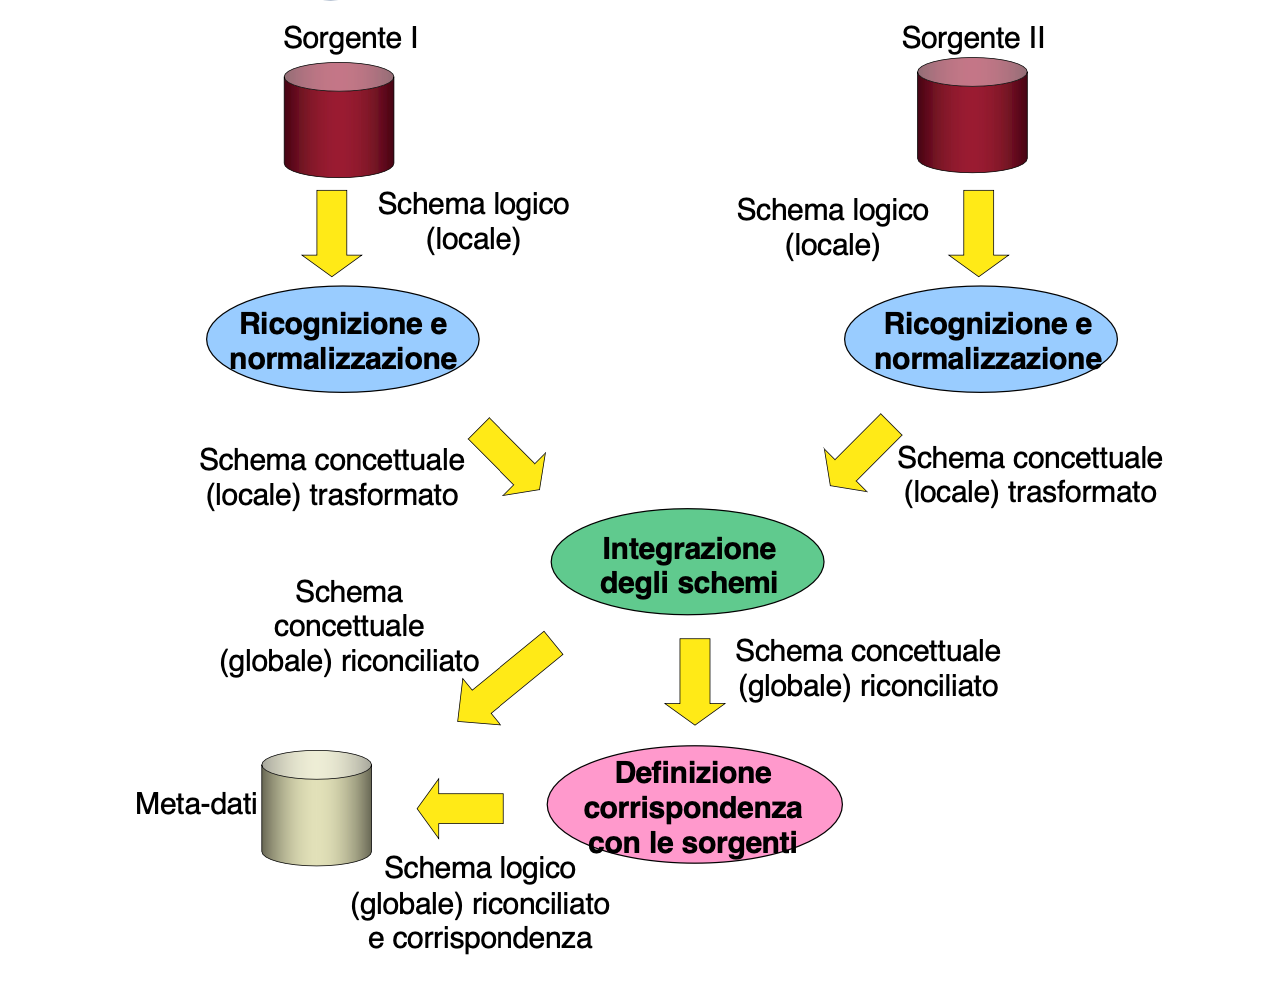
\includegraphics[width=0.7\linewidth]{img/analisi}
	\caption{Fase di analisi e riconciliazione}
	\label{fig:analisi}
\end{figure}
\subsubsection{Ricognizione e Normalizzazione}
\begin{itemize}
	\item
	\textbf{Ricognizione}: analisi approfondito degli schemi locali, guardo le tabelle e cerco di capire il significato di ciascuna tabella
	\item 
	\textbf{Normalizzazione}: significa che in teoria dovrei accorgermi che ci sono delle tabelle denormalizzate, cioè che ci sono delle dipendenze funzionali nascoste. 
\end{itemize}

\subsubsection{Analisi dei requisiti}
Qui l’obiettivo è raccogliere le esigenze di utilizzo del data mart espresse dai suoi utenti finali. Essa ha un’importanza fondamentale:
\begin{enumerate}
	\item 
	Perchè impatta in primis sullo schema concettuale
	\item 
	Specifiche per l'ETL legata alla sporcizia dei dati
	\item 
	Specifiche per l'analisi dei dati
\end{enumerate}
Ho due principali categorie di utenti:
\begin{itemize}
	\item 
	\textbf{Business Users}: persone che non sono tecniche. Usano il loro linguaggio, contraddicendosi tra di loro ma anche con sé stessi
	\item 
	\textbf{DBA}: in questo caso, i requisiti che dovranno essere catturati riguardano principalmente vincoli di varia natura imposti sul sistema di DW.
\end{itemize}
Per l’analisi dei requisiti bisogna preparare delle interviste indicendo delle riunioni, durante la quale si parla con i clienti. Ci sono due modi per strutturare un’intervista:
\begin{itemize}
	\item 
	\textbf{A piramide}: è un approccio di tipo induttivo, in cui l’intervistatore parte da domande molto dettagliate e progressivamente si allarga l’ambito della domanda. Questo tipo di approccio va bene con un intervistato scettico, che non si vuole far coinvolgere.
	\item
	\textbf{A imbuto}: si parte da domande più ampie e via via con domande più specifiche. Viene usato con un intervistato che è in soggezione. 
\end{itemize}
In qualunque modo si faccia l’analisi dei requisiti la cosa fondamentale è arrivare ad aver capito quali sono i fatti, in quando il fatto è la granularità (livello più spinto di dettaglio a cui voglio arrivare) giusta dell’informazione da catturare. A volte gli analisti fanno delle riunioni di analisi guidate dalle query, creando dei problemi, perché se chiedo agli utenti le query che vogliono fare, ottengo molte query e di conseguenza risulta difficile ottenere i fatti. Per ogni fatto occorre definire l’intervallo di storicizzazione, ovvero l’arco temporale che gli eventi memorizzati devono coprire. 
\subsubsection{Il carico di lavoro}
Il carico di lavoro OLAP è imprevedibile, ma è anche vero che il nucleo del carico di lavoro lo posso prevedere, perché ho già la reportistica statica, oltre quei report che l’utente ha già e che devono essere replicati nel nuovo cubo. In questa fase il carico di lavoro può essere espresso in linguaggio naturale; esso sarà comunque utile per valutare la granularità dei fatti e le misure d’interesse, nonché per iniziare ad affrontare il problema dell’aggregazione. 

Altri requisiti che vanno colti durante la fase di analisi sono legati alla periodicità dell’alimentazione (ogni quando deve fare l’ETL?) 
	
\section{Progettazione Concettuale}
Questa fase è di cruciale importanza poiché definisce il contenuto informativo del data mart. Tutta la prima parte di questa fase si occupa di capire qual è il modello che viene utilizzato, quindi individuare i vari costrutti che si potranno utilizzare. Non vi è uno standard ufficiale per la realizzazione della parte di progettazione concettuale del data mart. È possibile utilizzare il modello E-R per il data mart? No, perché è troppo espressivo e perché è nato per modellare realtà di business fatte in qualunque modo. Qui il modello deve essere multidimensionale e bisogna rispettare dei vincoli; quindi, ci devono essere gerarchie progettate in un certo modo. Molti progettisti disegnano direttamente gli schemi a stella (schemi logici relazionali). Questo tipo di approccio non è conveniente e funziona male perché racchiude solo la definizione di un insieme di relazioni e di vincoli di integrità (sono denormalizzate in pratica). 

Il formalismo che bisogna utilizzare si chiama \textbf{Dimensional Fact Model (DFM}). Ha una larga diffusione nei contesti italiani ed esteri, ma soprattutto nel mondo della ricerca. È un modello concettuale grafico pensato per:
\begin{itemize}
	\item 
	Supportare efficacemente il progetto concettuale
	\item 
	Permette di verificare che le interrogazioni (query OLAP) siano effettivamente esprimibili sul cubo che stiamo disegnando 
	\item 
	Supportare un dialogo tra progettista e utente finale
	\item 
	È fondamentale per la documentazione che deve essere espressiva e non ambigua
	\item 
	Creare una piattaforma stabile da cui partire per il progetto logico
\end{itemize}

Quando si utilizza il \textbf{DFM} creiamo degli schemi detti schemi di fatto. Trattandosi di schemi multidimensionali, ovviamente, disegneremo fatti, misure e gerarchie. Distingueremo la parte del DFM in costrutti di base e costrutti avanzati. I primi coprono un pò di più dell’espressività del modello multidimensionale. I secondi, invece, servono per modellare le sfumature che si incontrano nei progetti reali. 
\subsection{I costrutti di base}
\begin{itemize}
	\item
	\textbf{Fatto}: è un fenomeno di business che accade dinamicamente all’interno dell’azienda. È essenziale che un fatto abbia aspetti dinamici, ovvero evolva nel tempo
	\item 
	\textbf{Dimensione}: attributi numerici che quantificano il fatto da un certo punto di vista (il voto di laurea, qtà acquistata)
	\item 
	\textbf{Misura}: coordinate di accesso al cubo. 
\end{itemize}
\begin{figure}[H]
	\centering
	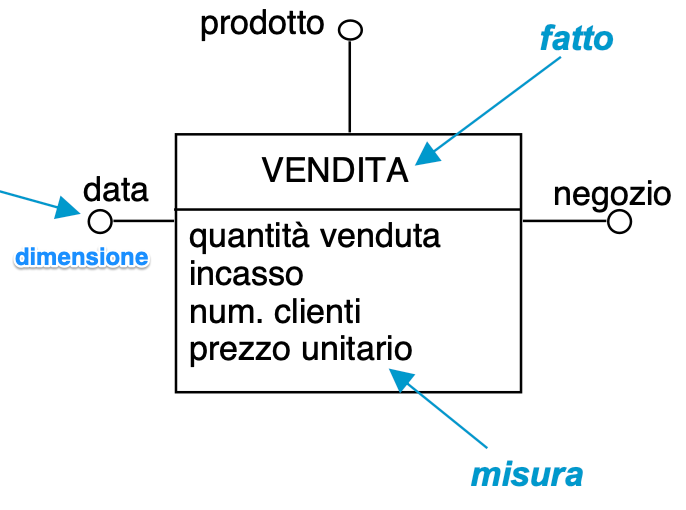
\includegraphics[width=0.7\linewidth]{img/example_fatto}
	\caption{Esempio di ...}
	\label{fig:exfatto}
\end{figure}
Quindi il tipo di relazione che ho tra prodotto, data e negozio è una classica associazione molti a molti. Dunque, un \textbf{fatto} esprime una associazione molti a molti tra le dimensioni.

Una \textbf{gerarchia} è una sequenza di attributi collegati tra di loro da associazioni molti ad uno, ossia da dipendenze funzionali. Le gerarchie non sono necessariamente dei percorsi, ma possono avere forme più complesse. In particolare possono essere degli alberi, i cui nodi si chiamano attributi dimensionali, i quali descrivono le dimensioni in modo via via più aggregato. L’\textbf{albero} non orientato è un grafo aciclico. In quest' albero la radice è la dimensione, mentre gli archi rappresentano dipendenze funzionali. 

Un \textbf{evento primario} è una particolare occorrenza di un fatto, individuata da una ennupla costituita da un valore per ciascuna dimensione. A ciascun evento primario è associato un valore per ciascuna misura. Per modellare il concetto dell’aggregazione sul DFM si ragiona in termini di group-by-set (livello di aggregazione) e di conseguenza aggrego (la sparsità diminuisce) nella query gli eventi primari in eventi secondari. Tanti eventi primari contribuiscono a costruire un evento secondario.  

Dato un DFM qualsiasi, in qualunque modo si scelga un sottoinsieme di attributi dimensionali, a patto che non ci siano dipendenze funzionali, ho un possibile group-by-set. 

\subsection{I costrutti avanzati}
\begin{itemize}
	\item 
	\textbf{Attributo descrittivo}: aggiunge delle informazioni su un attributo dimensionale, a cui è connesso da una associazione uno-a-uno. Questo tipo di attributi possono essere utilizzati per la selezione ma non possono essere utilizzati per l’aggregazione (non possono finire dentro ad un group-by-set). Gli attributi descrittivi non hanno figli. Posso discretizzare gli attributi descrittivi trasformandoli in un attributo dimensionale.  
	\item 
	\textbf{Archi opzionali}: è un arco molti-ad-uno ma entra in gioco la cardinalità minima. Con l’arco opzionale dico che per alcuni valori del padre non è definito nessun valore del figlio. 
		\begin{figure}[H]
		\centering
		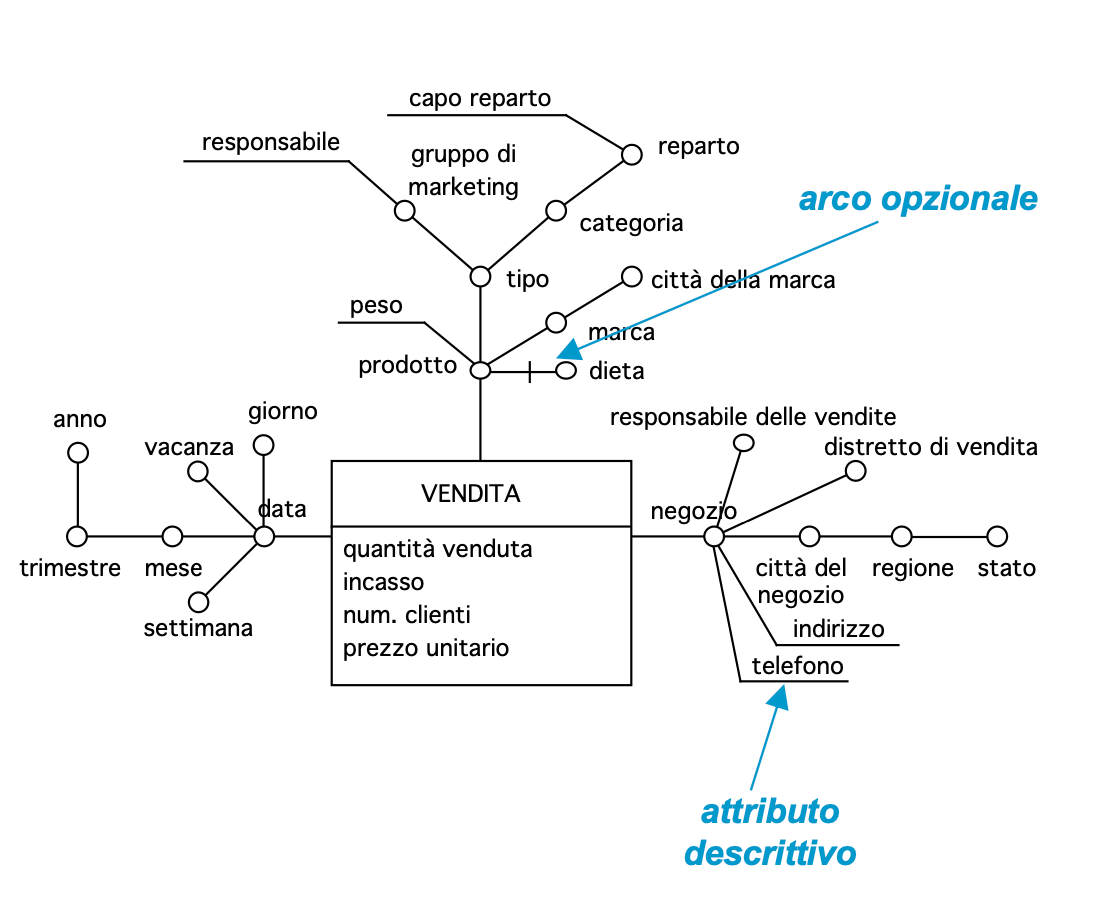
\includegraphics[width=0.6\linewidth]{img/descrittivo}
		\caption{Attributo descrittivo e arco opzionale}
		\label{fig:descr}
	\end{figure}
	\item 
	\textbf{Gerarchia condivisa}: in realtà le gerarchie possono avere dei cicli. Ho quattro modi per creare dei cicli nelle gerarchie del DFM, con quattro significati diversi. Il primo modo è la gerarchia condivisa, che è quello più debole, perché non pone vincoli sulle istanze. Una gerarchia condivisa è un albero che viene usato due o più volte all’interno dello stesso schema di fatto.
	\begin{figure}[H]
		\centering
		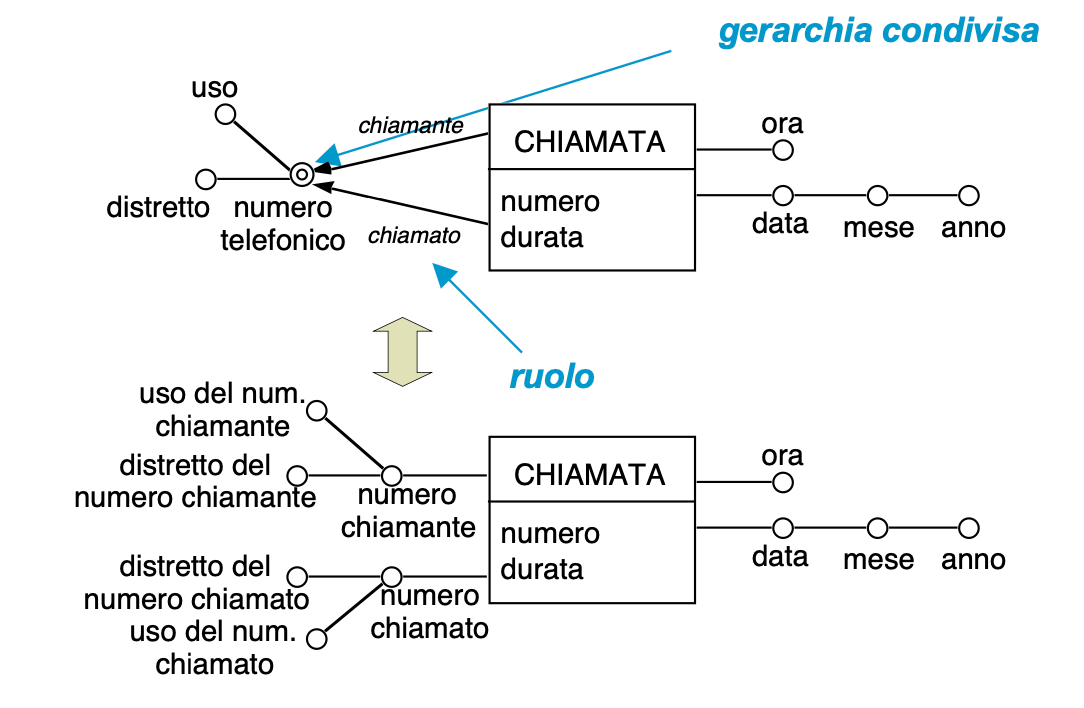
\includegraphics[width=0.6\linewidth]{img/condivisa}
		\caption{Gerarchia condivisa}
		\label{fig:condivisa}
	\end{figure}
	\item 
	\textbf{Convergenza}: aggiungo un vincolo sulle istanze. Mentre nel caso della condivisione non pongo vincoli sulle istanze, nel caso della convergenza non solo ho più percorsi che partono da un punto e arrivano nell’altro punto, ma qualunque dei due percorsi io prenda per ogni valore del punto di partenza arrivo sempre nello stesso punto di arrivo. Ho un vincolo aggiuntivo sulle istanze. 
	\begin{figure}[H]
		\centering
		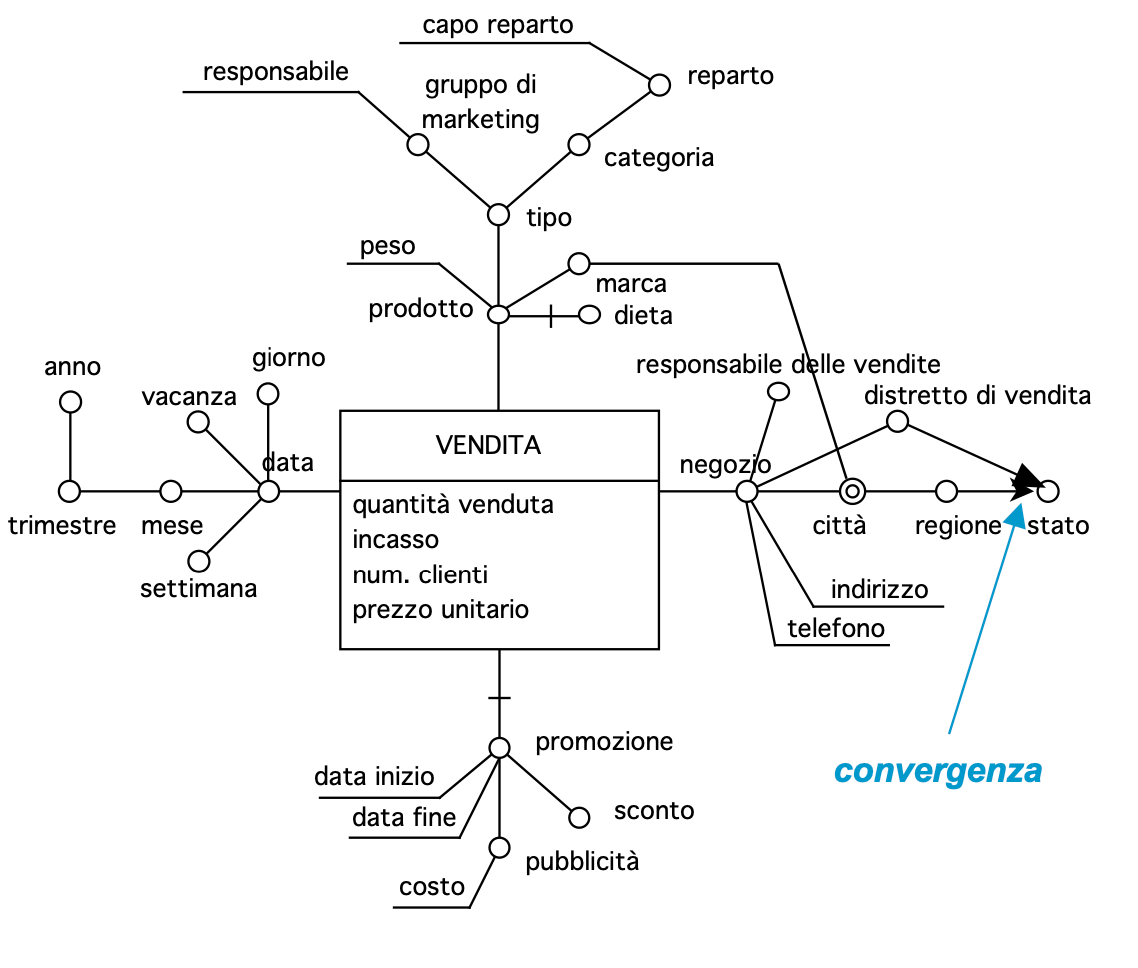
\includegraphics[width=0.6\linewidth]{img/convergenza}
		\caption{Convergenza}
		\label{fig:conv}
	\end{figure}
	\item 
	\textbf{Gerarchia incompleta}: per alcune istanze della gerarchia mancano dei valori di alcuni valori intermedi. La particolarità della gerarchia incompleta è che si hanno per le diverse istanze della gerarchia, un numero variabili di livelli pieni. 
		\begin{figure}[H]
		\centering
		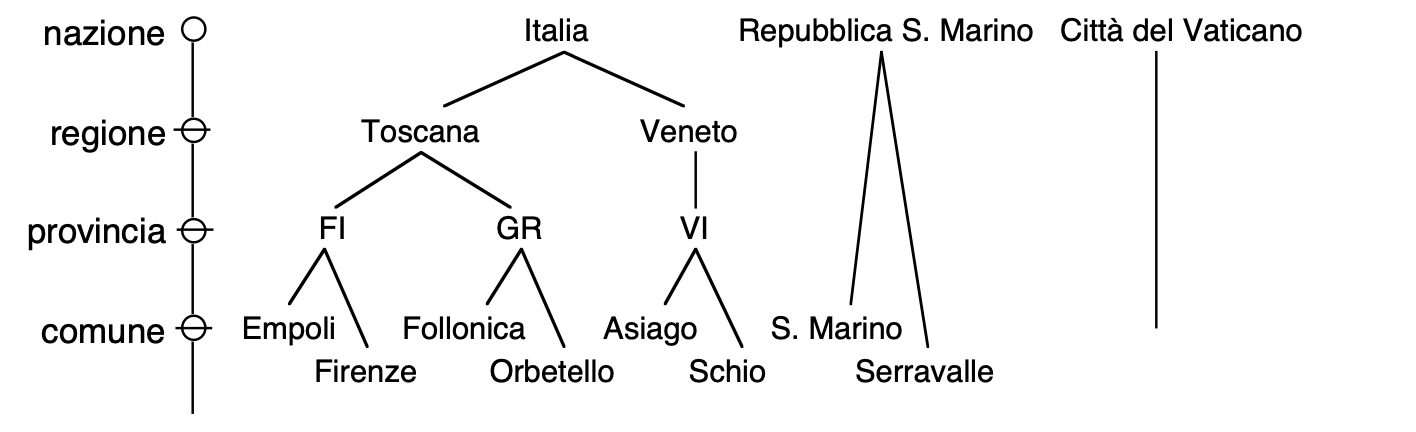
\includegraphics[width=0.7\linewidth]{img/incompleta}
		\caption{Gerarchia incompleta}
		\label{fig:incompleta}
	\end{figure}
	\item 
	\textbf{Additività}: esprime in che modo le misure possono essere aggregate. Di per sé le misure sono classificabili in tre categorie:
	\begin{itemize}
		\item 
		\textbf{Misure di flusso}: si riferiscono ad un periodo di tempo e vengono istanziate in modo cumulativo (il numero di prodotti venduti in un giorno, l’incasso mensile, il numero di nati in un anno). Sono quelle più semplice da gestire perché sono additive lungo tutte le dimensioni.
		\item 
		\textbf{Misure di livello}: vengono valutate in istanti di tempo (il numero di prodotti in inventario, il numero di abitanti di una città)
		\item 
		\textbf{Misure unitarie}: vengono valutate in particolari istanti di tempo, ma sono espresse in termini relativi (il prezzo unitario di un prodotto, la percentuale di scoto, il cambio di una valuta) 
	\end{itemize}
	
	
	La misura è detta \textbf{additiva} lungo una dimensione se i suoi valori possono essere aggregati lungo la corrispondente gerarchia tramite l’operatore di somma, altrimenti è detta non-additiva. Una misura \textbf{non-additiva} è non-aggregabile se nessun operatore di aggregazione può essere usato su di essa.  
	
	Uno schema di fatto si dice \textbf{vuoto} se non ha misure. In questo caso, il fatto registra solo il verificarsi di un evento.
\end{itemize}
	
	\subsection{Editing dell'albero}
	 Ci si accorge che alcuni attributi dell’albero non sono d’interesse per l’analisi. L’eliminazione del nodo si può fare in due modi:
	 \begin{itemize}
	 	\item 
	 	\textbf{Potatura}: taglio quel nodo e tutti i suoi figli
	 	\item 
	 	\textbf{Innesto}: si elimina un nodo mantenendo i suoi figli
	\end{itemize}
	 L’innesto deriva dalla teoria delle dipendenze funzionali. Quando un \textbf{vertice opzionale} viene innestato, tutti i suoi figli ereditano il trattino di opzionalità. Nel caso di potatura o innesto di un vertice opzionale v con padre "v’" è possibile aggiungere a "v’" un nuovo figlio "b" corrispondente a un attributo booleano che esprima l’opzionalità. 
	 
	 Tutte le volte  che durante l’editing si decida di eliminare un attributo che è un figlio diretto della radice e fa parte della chiave della relazione che si è scelto come fatto oppure fa parte dell’identificatore dell’entità che si è scelto come fatto si sta cambiando la granularità. 
	 
	 Nella pratica possono rendersi necessarie ulteriori manipolazioni sull’albero degli attributi:
	 \begin{itemize}
	 	\item
	 	può essere necessario modificarne radicalmente la struttura sostituendo il padre di un certo nodo: ciò corrisponde ad aggiungere o eliminare una dipendenza funzionale. 
	 	\begin{figure}[H]
			\centering
			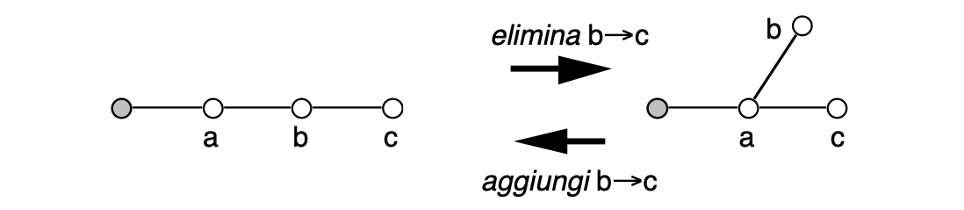
\includegraphics[width=0.6\linewidth]{img/editing}
			\caption{Editing dell'albero}
			\label{fig:editing}
	 	\end{figure}
 	Perché dovrei aggiungere o togliere una dipendenza funzionale? Aggiungere una dipendenza funzionale conviene se lo schema sorgente non è perfettamente normalizzato.
 	
 	A volte ci capiterà di eliminare delle dipendenze funzionali. L’unico caso è quando dobbiamo scegliere come misura un attributo che non è figlio diretto della radice. 
	 	\item 
	 	può capitare che dentro l’albero ci finiscano degli archi che rappresentano dei casi particolari di associazioni molti a uno, ovvero associazioni uno-a-uno. Questo può succedere in più situazioni: se partiamo da un E/R in cui abbiamo gerarchie di specializzazione, la gerarchia da luogo ad associazioni binarie uno-a-uno. Nell’E/R di partenza può capitare che si abbia già un’associazione uno-a-uno (esempio iscritto e tessera in palestra). Dentro il DFM non si possono avere archi tra due attributi dimensionali che rappresentano associazioni uno-a-uno, ma sempre molti-a-uno. 
	 	
	 	In presenza di un’associazione uno-a-uno sono consigliabili due soluzioni:
	 	\begin{itemize}
	 		\item 
	 		quando il vertice v determinato dall’associazione uno-a-uno ha dei discendenti di interesse lo si può eliminare dall’albero tramite innesto
	 		\item 
	 		quando v non ha discendenti di interesse lo si può rappresentare come attributo descrittivo
	 		\item 
	 		in alcuni casi può convenire invertire i due nodi coinvolti
	 	\end{itemize}

	 \end{itemize}
 
 \subsection{Scelta delle dimensioni}
 Le \textbf{dimensioni} vanno scelte tra i figli diretti della radice e devono corrispondere ad attributi che abbiamo un dominio finito e discreto. La loro scelta è cruciale per il progetto poiché definisce la granularità degli eventi primari. 
\subsection{Scelta delle misure}
Le \textbf{misure} sono i figli diretti della radice che non abbiamo scelto come dimensioni. Sono sempre attributi numerici (reali o interi). 
\subsection{Creazione dello schema di fatto} 
L’albero degli attributi può essere tradotto in uno schema di fatto che include le dimensioni e misure definite:
\begin{itemize}
	\item 
	le gerarchie corrispondono ai sottoalberi dell’albero degli attributi con radice nelle diverse dimensioni
	\item 
	il nome del fatto corrisponde al nome dell’entità scelta come fatto
	\item 
	è possibile potare e innestare l’albero per eliminare dettagli inutili
	\item 
	è possibile aggiungere attributi dimensionali definendo opportuni intervalli per attributi numerici
	\item 
	gli attributi che non verranno usati per l’aggregazione possono essere contrassegnati come descrittivi; tra questi compariranno in genere anche gli attributi determinati da associazioni uno-a-uno e privi di discendenti
	\item 
	per quanto riguarda eventuali attributi alfanumerici figli della radice ma non prescelti né come dimensioni né come misure:
	\begin{itemize}
		\item 
		se la granularità degli eventi primari coincide con quella dell’entità F, essi possono essere rappresentati come attributi descrittivi associati direttamente al fatto, di cui descriveranno ciascuna occorrenza
		\item 
		se invece le due granularità sono differenti, essi devono necessariamente essere potati
	\end{itemize}
\subsection{Carico di lavoro e volume dati}
Per il data mart si hanno diversi schemi di fatto che mostrano il contenuto informativo del data mart dal punto di vista concettuale indipendente dall’implementazione. Il prossimo passo sarà tradurre gli schemi concettuali in schemi logici (ROLAP). È opportuno fare un ragionamento sul carico di lavoro e volume dati. Il carico di lavoro indica le query che più frequentemente verranno sottoposte al sistema. Per definizione il carico di lavoro OLAP è estemporaneo, ma il nucleo del carico di lavoro si può prevedere. La query OLAP standard ha una clausola di group-by, richiede una o più misure, e ha delle clausole di selezione. 

Quindi durante questa fase inizio a organizzare tutte le query che ho catturato duramente l’analisi dei requisiti, verificano che siano supportati dagli schemi concettuali che ho disegnato e comincio a legarle agli utenti. Per gestire la variabilità del carico di lavoro bisogna fare un monitoraggio costante. Non tutte le query possono essere lanciate da tutti gli utenti, quindi si comincia con la profilazione, ovvero capire quali saranno i principali profili di utenti che dovranno accedere al data mart. Comincio con il legare quindi a ciascun utente dell’aree di analisi che potrebbero essere utili. Devo spiegare per tutti gli utenti di ciascun profilo quali query potranno formulare. In questa fase è importante anche cominciare a misurare il volume dati. Misurare il volume dati significa per ciascun attributo che si ha nella gerarchia capire qual è la sua cardinalità di dominio. 

\end{itemize}



\end{document}